\documentclass[a4paper,12pt]{article}
\usepackage[utf8]{inputenc}
\usepackage[T1]{fontenc}
\usepackage[hungarian]{babel}
\usepackage{graphicx}
\usepackage{geometry}
\geometry{a4paper,
		     tmargin = 35mm, 
		     lmargin = 30mm,
		     rmargin = 30mm,
		     bmargin = 30mm}
\usepackage{mathtools}
\usepackage{amsmath}
\usepackage{color}
\usepackage{setspace}
\usepackage{amsmath,amssymb}
\usepackage{float}

%Define double underlining
\def\doubleunderline#1{\underline{\underline{#1}}}
% To change the abstract name from the overridden `Kivonat` to `Bevezetés`
\addto{\captionshungarian}{\renewcommand{\abstractname}{Bevezetés}}
% Section numbering
\renewcommand\thesection{\Roman{section}}
%\renewcommand\thesubsection{\thesection.\roman{subsection}}

% Laplace and D'Alambert operators
\newcommand*\Laplace{\mathop{}\!\mathbin\bigtriangleup}
\newcommand*\DAlambert{\mathop{}\!\mathbin\Box}

%Vector
\makeatletter
\newcommand{\Spvek}[2][r]{%
  \gdef\@VORNE{1}
  \left(\hskip-\arraycolsep%
    \begin{array}{#1}\vekSp@lten{#2}\end{array}%
  \hskip-\arraycolsep\right)}

\def\vekSp@lten#1{\xvekSp@lten#1;vekL@stLine;}
\def\vekL@stLine{vekL@stLine}
\def\xvekSp@lten#1;{\def\temp{#1}%
  \ifx\temp\vekL@stLine
  \else
    \ifnum\@VORNE=1\gdef\@VORNE{0}
    \else\@arraycr\fi%
    #1%
    \expandafter\xvekSp@lten
  \fi}
\makeatother

\begin{document}

\linespread{1.2}

\begin{titlepage}
% Template for future notes.

	\centering
	
\includegraphics[width=0.66\textwidth]{elte.jpg}\par\vspace{1cm}
	{\scshape\LARGE ELTE TTK \par}
	\vspace{2cm}
	{\scshape\Large Az általános relativitáselmélet alapjai\par}
	\vspace{1.5cm}
	{\large\itshape készült az előadások alapján, írta: \par}
	\vspace{1cm}
	{\large\itshape Olar Alex\par}
	\vfill
	oktató\par
	\vspace{0.5cm}
	{\Large Dávid Gyula, \itshape{dgy}}

	\vfill

% Bottom of the page
	{\large 2016/2017 \par}
\end{titlepage}
%%%%%%%%%%%%%%%%%%%%%

\begin{abstract}
Ez a jegyzet \itshape{Dávid Gyula} előadássorozata alapján készült a 2016/17-es tanév második féléveben. A jegyzet bővítése tervben van. Az előadássorozat 3 féléven keresztül végig kíséri a most II. évfolyamot egészen a BSc végéig. Ezen összefoglaló célja számomra az ismétlés, majd közkinccsé tétel. 
\end{abstract}

\vfill

\tableofcontents

\newpage
%%%%%%%%%%%%%%%%%%%%%

\section{ Jelölések}
\vspace{1cm}
\hspace{0.5cm} A speciális relativitáselmélet kurzusról ismert jelölésekhez hasonlóan felső és alsó indexeket használunk majd. Ha az index az angol ABC betűje, akkor az 0-3 közötti számozást jelent, ha a görög ABC betűje, akkor csak 1-3 között indexel.
\newline
\begin{center}
$x^{k} = \Spvek{ct;x;y;z} \quad x_{k} = \Spvek{ct;-x;-y;-z} \quad x^{\alpha} = \Spvek{x;y;z} \quad x_{\alpha} = \Spvek{x;y;z}$
\end{center}
\hspace{0.5cm} A tenzorok indexelése hasonlóan felső, alsó, vegyes indexekkel történik.
\begin{center}
$\Lambda^{i j} \quad \Lambda_{i j} \quad \Lambda^{i}_{j}$
\end{center}

\newpage
%%%%%%%%%%%%%%%%%%%%%

\section{ Speciális relativitáselmélet - áttekintés}
\vspace{0.5cm} Minden objektum szimmetria csoportjába tartozó transzformációk a:
\begin{itemize}
\item eltolás $\rightarrow$ impulzus megmaradás
\item Lorentz-boost
\item időbeli eltolás $\rightarrow$ energia megmaradás
\item forgatás $\rightarrow$ impulzusmomentum megmaradás
\end{itemize}

\vspace{0.5cm} Az $x^{k}$ koordináták transzformációja ezen szimmetriák alkalmazása.
\begin{equation*}
x'^{k} = \Lambda^{k}_{l}x^{l} + a^{k}
\end{equation*}
\vspace{0.5cm} Ahol $a^{k}$ egy konstans eltolás, míg a két indexes tenzor a Lorentz-transzformációt írja le, a következő alakban:
\begin{equation*}
\Lambda = \left(\begin{array}{cccc} \pm 1&0&0&0 \\ 0& && \\ 0 &&\it{\Large{I}} &\\ 0 && & \end{array}\right)
\left(\begin{array}{cccc} 1&0&0&0 \\ 0& & & \\ 0 & & \it{\large{F}} &\\ 0 &&&  \end{array}\right)
\left(\begin{array}{cccc} \cosh{\chi}&&-\underline{\tilde{n}}\sinh{\chi}& \\ &  && \\ -\underline{n}\sinh{\chi}&&\it{\large{I + (\cosh{\chi} - 1)\underline{n}\circ \underline{n}}}&\\ && & \end{array}\right)
\end{equation*}
\newline
Ahol $I$, $F$ rendre a 3 dimenziós egység és forgás mátrixok.  \newline
\hspace{1cm}
\vspace{0.5cm} A speciális relativitáselméletben a metrikus tenzor rendezi át az indexeket. Ezzel értelmezett a skaláris szorzás is a négyesvektorok között.
\begin{equation*}
x_{k} = g_{kl}x^{l} \quad x^{k} = g^{kl}x_{l} \quad g^{kl}g_{lm} = \delta^{k}_{m}
\end{equation*}
\vspace{0.5cm} A speciális relativitáselméletben a metrikus tenzor saját magának az inverze, konstans.
\begin{equation*}
g_{kl} = \left(\begin{array}{cccc} 1&0&0&0\\ 0&-1&0&0\\ 0&0&-1&0\\0&0&0&-1 \end{array}\right)
\end{equation*}
\vspace{0.5cm} Az ezzel definiált skalárszorzás pedig.
\begin{equation*}
x^{k}x_{k} = g_{kl}x^{k}x^{l} = (ct)^{2} - x^{2} - y^{2} - z^{2}
\end{equation*}
Az általános relativitáselmélet célja, hogy lokálisan teljesítse a speciális relativitáselméletet, viszont globálisan egy új leírást adjon a világra.
\newpage
%%%%%%%%%%%%%%%%%%%%%%%%%

\section{ Newtoni - gravitáció}
A newtoni gravitáció elmélete az évszázadok során beleivódott minden ember tudatába. A távolba hatás, a távoli testek által egymásra kifejtett erő mind-mind alapfogalmak a fizika tanulás kezdetén. \newline
A mozgásegyenletekben szereplő arányossági tényezők egyenlősége komoly mérési eljárások kidolgozásra révén volt bizonyítható, súlyos tömeg, tehetetlen tömeg.
\begin{equation*}
m_{t}\vec{a} = m_{s}\vec{g}(\vec{r},t)
\end{equation*}
Kísérleti tény az is, hogy zárt görbén a gravitációs erőnek nincsen munkája. Azaz:
\begin{equation*}
\oint_\gamma \vec{g}(\vec{r},t) \,d\vec{r} = 0 = \int_F (\nabla \times \vec{g}) d\vec{F} = 0 \quad \quad \rightarrow \quad \quad \nabla \times \vec{g} = \vec{0}
\end{equation*}
Ebből következik, hogy $\vec{g}$ egy skalármező negatív gradienseként előállítható. Így:
\begin{equation*}
\oint_{\partial V} \vec{g} d\vec{F} = \int  \nabla\vec{g}dV = - 4\pi G \int \rho(\vec{r})dV \quad \rightarrow \quad \nabla\vec{g} = -4\pi G\rho(\vec{r})
\end{equation*}
Így látható, hogy folytonos tömegeloszlásra a Newton-féle gravitációs törvény a következő alakot ölti.
\begin{equation*}
\vec{g} = -\nabla\Phi \quad \rightarrow \quad \Laplace\Phi = 4\pi G \rho(\vec{r})
\end{equation*}
Az utóbbi lényegében a gravitációra felírt Poisson-egyenlet. \newline
\hspace{0.5cm} Áttérve a speciális relativitáselméletre a gravitációs erő általánosítása a következő egyenlet lenne:
\begin{equation*}
\frac{d}{d\tau}(Mu_{k}) = M \partial_{k}\Phi
\end{equation*}
A sajátidő ($\tau$) szerinti deriválást elvégezve és kihasználva, hogy a négyessebesség $u_{k}u^{k} = c^{2}$ a következő összefüggést kapjuk:
\begin{equation*}
\frac{dM}{d\tau}c^{2} = \frac{\partial \Phi}{\partial x^{k}} \frac{dx^{k}}{d\tau}M = \frac{d\Phi}{d\tau}M
\end{equation*}
Ezt nevezhetjük a \textsc{Novobátzky-effektus}  speciális esetének. Mivel ez egy szeparálható differenciál egyenlet, a megoldása előáll
\begin{align*}
M = m e^{\frac{\Phi(x^{k})}{c^{2}}}
\end{align*}
Ezt pedig $1911$-ben \textsc{Nordström} vezette le. Lényegében ez volt a legjobb gravitáció elmélet amit a speciális relativitáselmélet előállított. A korábbiak alapján a mozgásegyenlet is előállítható, ha a kezdeti egyenletbe visszahelyettesítjük a $\frac{dM}{d\tau}$ tagot.
\begin{equation*}
\frac{dM}{d\tau} = \frac{1}{c^{2}}Mu^{l}\partial_{l}\Phi \quad \rightarrow \quad (\delta^{l}_{k} - \frac{u^{k}u_{l}}{c^{2}})\partial_{l}\Phi = \frac{du_{k}}{d\tau}
\end{equation*}
Jól látható, hogy a potenciál gradiense előtt álló operátor egy, a négyessebességre merőleges vetítést hajt végre.
\section{ Alapfogalmak}
\hspace{0.5cm} Az első féléves mechanika és az Elméleti mechanika tárgyak szerves részét képezi a gyorsuló koordináta-rendszerek vizsgálata. Mind ismerjük a kulcsfogalmakat. Szükség van egy rögzített koordináta-rendszerre amihez képest egy másik origója $a_{0}$ gyorsulással transzlációt végezhet és foroghat. A forgás leírására a koordináta-rendszerek közötti ortogonális transzformációt használjuk, ahol az ortogonális mátrixok időfüggőek.
\begin{equation*}
\doubleunderline{\dot{O}}\hspace{0.1cm}\doubleunderline{O}^{T} = \doubleunderline{\Omega} = \underline{\omega} \times
\end{equation*}
A mozgásegyenlet pedig a következőképen transzformálódik:
\begin{equation*}
m\underline{a} = \underline{F} + m\underline{a}_{0} + m \underline{\omega} \times (\underline{\omega} \times \underline{r}) + 2m\underline{\omega}\times\underline{\dot{r}} + m \underline{\dot{\omega}}\times \underline{r}
\end{equation*}
\textsc{Einstein} arra jött rá, hogy a gravitáció sem erő, hanem egy koordináta transzformációval eltüntethető jelenség. Ennek leírására segítséget kért egy Magyarországon született, matematikus barátjától, \textsc{Marcell Grossmann}tól. Együtt dolgozták ki az általános relativitáselmélet matematikáját a \textsc{Riemann-féle differenciálgeometria} alapján. \newline
\par A kulcsgondolatok:
\begin{itemize}
\item Nincs globális koordináta-rendszer amihez viszonyítani lehetne a lokális rendszereinket.
\item Lokális rendszereink Minkowski-geometriájúak, azaz lokálisan a speciális relativitáselmélet teljesül.
\end{itemize}
\par
Ennek precíz matematikai leírásához a következő gondolati lépesek lennének szükségesek:
\begin{enumerate}
\item halmaz $\rightarrow$ ezen értelmezett folytonosság, differenciálhatóság
\item konnexió (kapcsolat a topologikus tér és a metrikus tér között)
\item metrika
\end{enumerate}
A leíráshoz a sokaságok elméletét fogjuk alapul venni. Ezek közül is nekünk a differenciálható részsokaságok egy speciális részhalmaza kell majd a tér-idő leíráshoz. Hiszen mit tud egy fizikus? \textsc{Deriválni.}
\subsection{ Affin tér:}
Egy affin tér egy (V, \textbf{V}, \textbf{-}) hármas, ahol:
\begin{itemize}
\item V nem üres halmaz
\item \textbf{V} vektortér
\item ''\textbf{-}'' leképezés pedig V  $\times$ V $\rightarrow$ \textbf{V}, amit (x,y) $\mapsto$ x-y = $\vec{a}$ alakban írunk
\end{itemize}
Axiómái a következők:
\begin{itemize}
\item (x-y) + (y-z) + (z-x) = $\vec{0}$
\item az affin tér és az alul fekvő vektortér dimenziója azonos
\item $\vec{a}$ = A \textbf{-} $o$ leképezést az affin tér $o$ középpontú ortogonalizációjának nevezzük
\end{itemize}
A tér-időről kezdetben csak annyit feltételezünk, hogy az egy 4 dimenziós affin tér, amely lokálisan Minkowski-struktúrával van ellátva. Ezeket a különböző rendszereket kell majd valahogy összefésülni.
\subsection{ Metrika}
\par Legyenek $a$,$b$ egy $\textsl{M}$ halmaz elemei. Ekkor a $\rho : \textsl{M} \times \textsl{M} \rightarrow \textsl{R}$ hozzárendelést metrikának nevezzük, ha:
\begin{itemize}
\item $\rho(a,b) \geq 0$, valamint akkor és csak akkor $0$, ha $a = b$
\item $\rho(a,b) = \rho(b,a)$
\item $\rho(a,b) \leq \rho(b,c) + \rho(c,a)$
\end{itemize}
\par A sokaságok leírásához viszont egyenlőre nem metrikát használunk. Mások lesznek az alapfogalmaink. A $\textsc{nyílt halmaz}$ok lesznek az alapfogalmaink. Erre építünk majd mindent, még ha nem is a lehető legprecízebb módon. Az $\textsl{Analízis I.}$ kurzusról már ismeretesek a nyílt halamzokra vonatkozó alapállítások:
\begin{itemize}
\item Végtelen sok nyílt halmaz uniója nyílt.
\item Véges sok nyílt halmaz metszete is nyílt.
\end{itemize}
\par Legyen $X$ egy halmaz, ennek nyílt részhalmazai $B$-k. Az ezeket tartalmzó struktúrát ekkor $\textsc{topologikus tér}$nek nevezzük, ha tartalmazza $X$-et, az üres halmazt, valamint a nyílt halmazok végtelen unióját és véges metszetét. A topologikus tér ezáltal egy olyan halmaz, amin a folytonosság értelmezve van, hiszen tudunk közelséget/szomszédságot definiálni. Gyakorlatban persze a fizikus nem absztrahál ennyire, visszanyúl a koordinátázáshoz.
\par Vegyünk egy sokaságot, legyen ez $\textsl{M}$. Ennek két részhalmazát $U$,$V$, melyek metszete nem üres képezzük le egy  rendre $p$,$q$: $\textsl{M}$  $\rightarrow$ $\textsl{$R^{n}$}$ paraméterezésekkel. Ekkor a közös metszet leképződött $\textsl{$R^{n}$}$ két részhalmazára amik között értelmezhető egy $F$ : $\textsl{$R^{n}$}$ $\rightarrow$ $\textsl{$R^{n}$}$ leképezés, amit kiterjeszthetünk $U$-ról, $V$-re, feltéve, hogy a paraméterezések invertálhatóak. Tehát $p$$\circ$ $F$ $\circ$ $q^{-1}$ : $U$$\rightarrow$ $V$ függvény már a sokaságon értelmezett. Megmutatható, hogy ez a paraméterezéstől független. 
\par Az ilyen leképzésesekkel értelmezhető az absztrakt sokaságon a folytonosság és deriválhatóság, hiszen $F$-en már ezeket könnyedén tudjuk értelmezni. A keletkezett térkép lapok maguk fölé definiálnak egy sokaságot, amit $\textsc{algebrai topológiának}$ nevezünk. Értelmezhetővé válik a differenciálható sokaság fogalom. Tartsuk szem előtt, hogy $\textsl{továbbra sincsen beágyazó tér}$ (matematikusok belátták, hogy nem triviális módon értelmezhető olyan tér, amibe beágyazható egy ilyen struktúra, de ez közelében sincs a hétköznapi fogalmainknak). 
\newline
\begin{center}
\par $\textit{Eljutottunk tehát oda, hogy ki tudjuk mondani, hogy a $\textsc{téridő modell}$ünk egy}$ \newline $\textit{olyan $4$ dimenziós differenciálható sokaság, amely lokálisan Minkowski-tér.}$
\end{center}
\par Az általános relativitáselméletben csakis felső indexes ''vektrok'' lesznek, mivel ezek a görbevonalú koordinátázáshoz képest, nem vektrokomponensek, hanem pusztán $\textsc{koordináták}$. Tehát nem transzformálódnak homogén lineáris módon.
\par Már értelmezhetünk skalármezőt is. Általánosságban csak mezőket tudunk majd értelmezni amúgy is, hiszen az elmélet csak a sokaság minden pontjában értelmezett objektumokat enged meg. Legyen tehát $\Phi : \textsl{M} \rightarrow \textsl{R}$, mivel $\textsl{P}$ pont kölcsönös egyértelmű viszonyba hoszható a térképzeésen egy $x^{k}$ koordinátával így a (fizikus módon ugyan azzal a betűvel jelölve) $\Phi : \textsl{$R^{n}$} \rightarrow \textsl{R}$ függvény már egy skalármezőt definiál $\textsl{M}$-n is.
\newline
\par $\textsl{Einstein}$ célja a gyorsuló koordinátákra való kovariáns áttérés matematikai leírása és fizikai megalapozása volt.
\par Ha ugyan arról a részsokaságról készítünk különböző térképzeéseket, akkor azok között léteznie kell egy folytonos, differenciállható és invertálható leképzésnek, ami ezeket egymásba transzformálja.
\section{ Topológia, derivációk, metrika}
\par Legyen a sokaság minden pontjában értelmezve egy $T_{p}$ vektortér ( - érintőtér - ), ami független a paraméterezéstől mégis annak segítségével definiálhatjuk, hiszen ezeket a paraméterezés deriváltjának az értékkészletének egy részén értelmezhetjük:
\begin{equation}
T_{P}(\textsl{M}) := Ran_{Dp(p^{-1}(x))}
\end{equation}
Az ezen pontokban vett érintőterek unióját $\textsc{tangens nyaláb}$nak nevezzük. Ennek $\textsl{szelése}$ egy vektormező, ami lényegében egy olyan művelet, ami minden ponthoz hozzárendel az adott pontban vett érintőtérből egy elemet. Mivel a vektromező minden egyes eleme más halamzból került ki, így a különböző lineáris terek közötti átszámítás nem triviális. Egy szemléltetést segítő ábra erről:
\begin{figure}[H]
\centering
\begin{minipage}{0.46\linewidth}
\centering
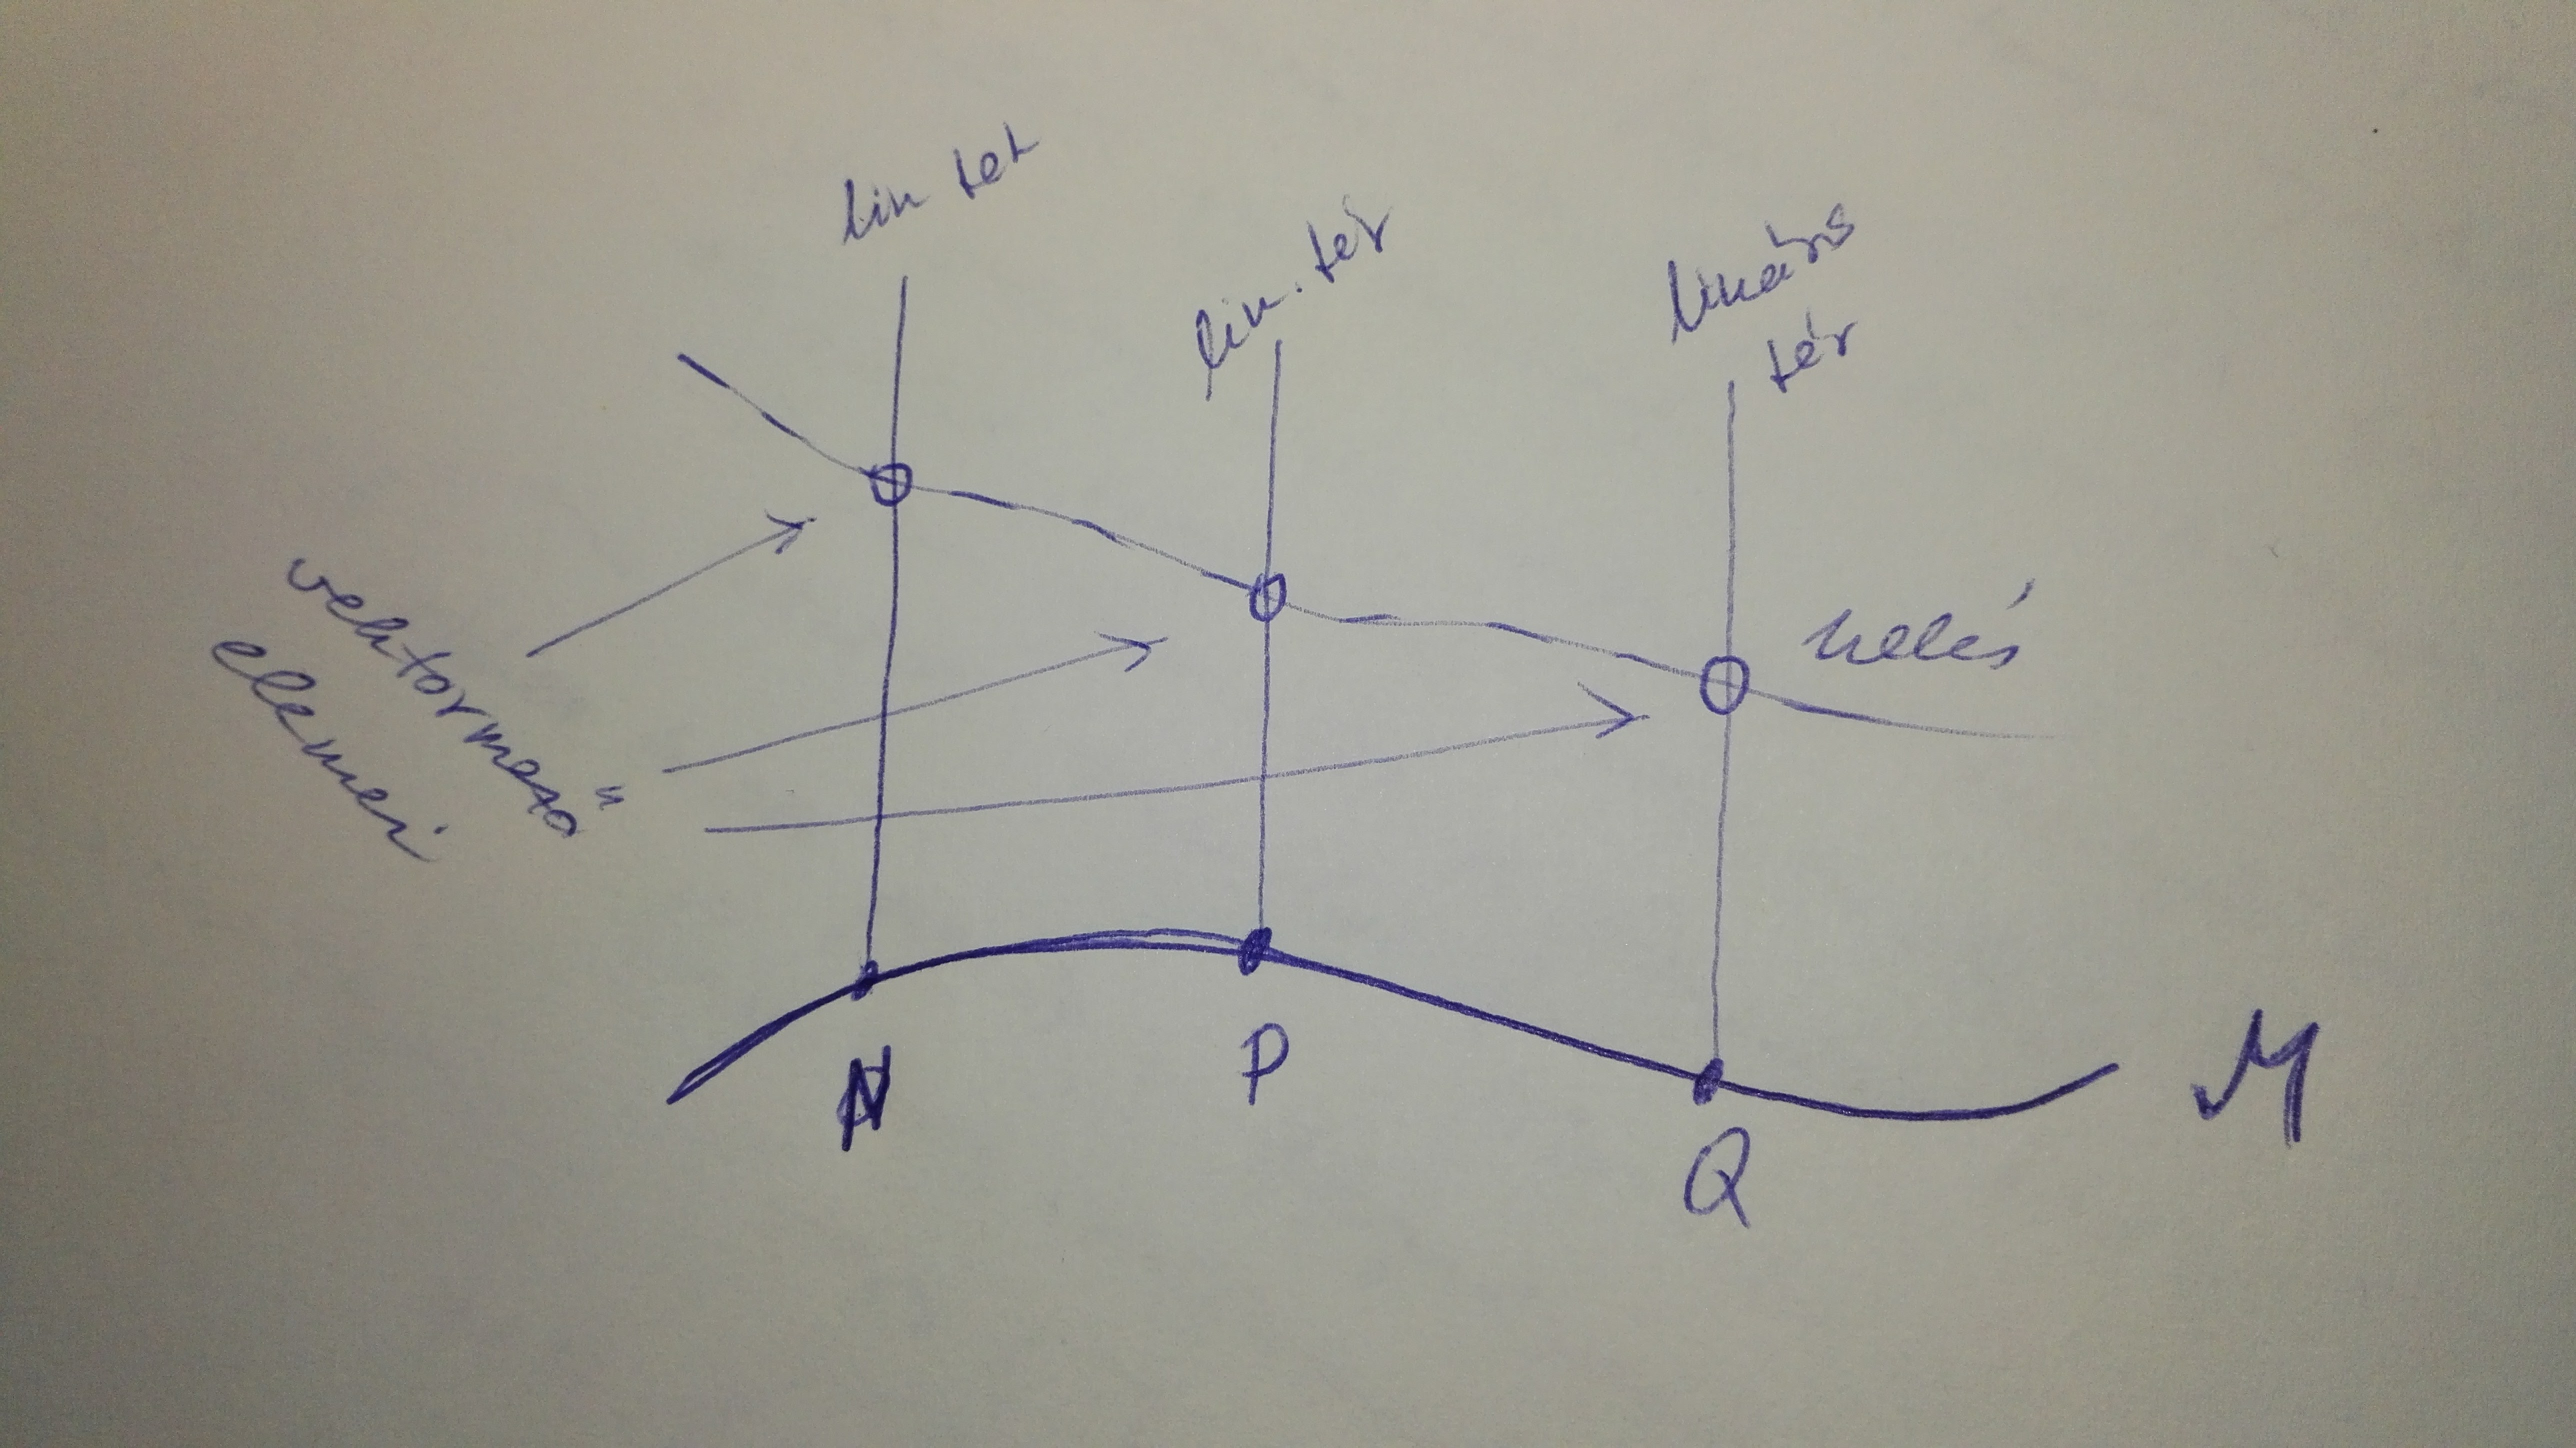
\includegraphics[width=0.9\linewidth]{szeles.jpg}
\caption{Szelés szemléltetése}
\end{minipage}
\begin{minipage}{0.46\linewidth}
\centering
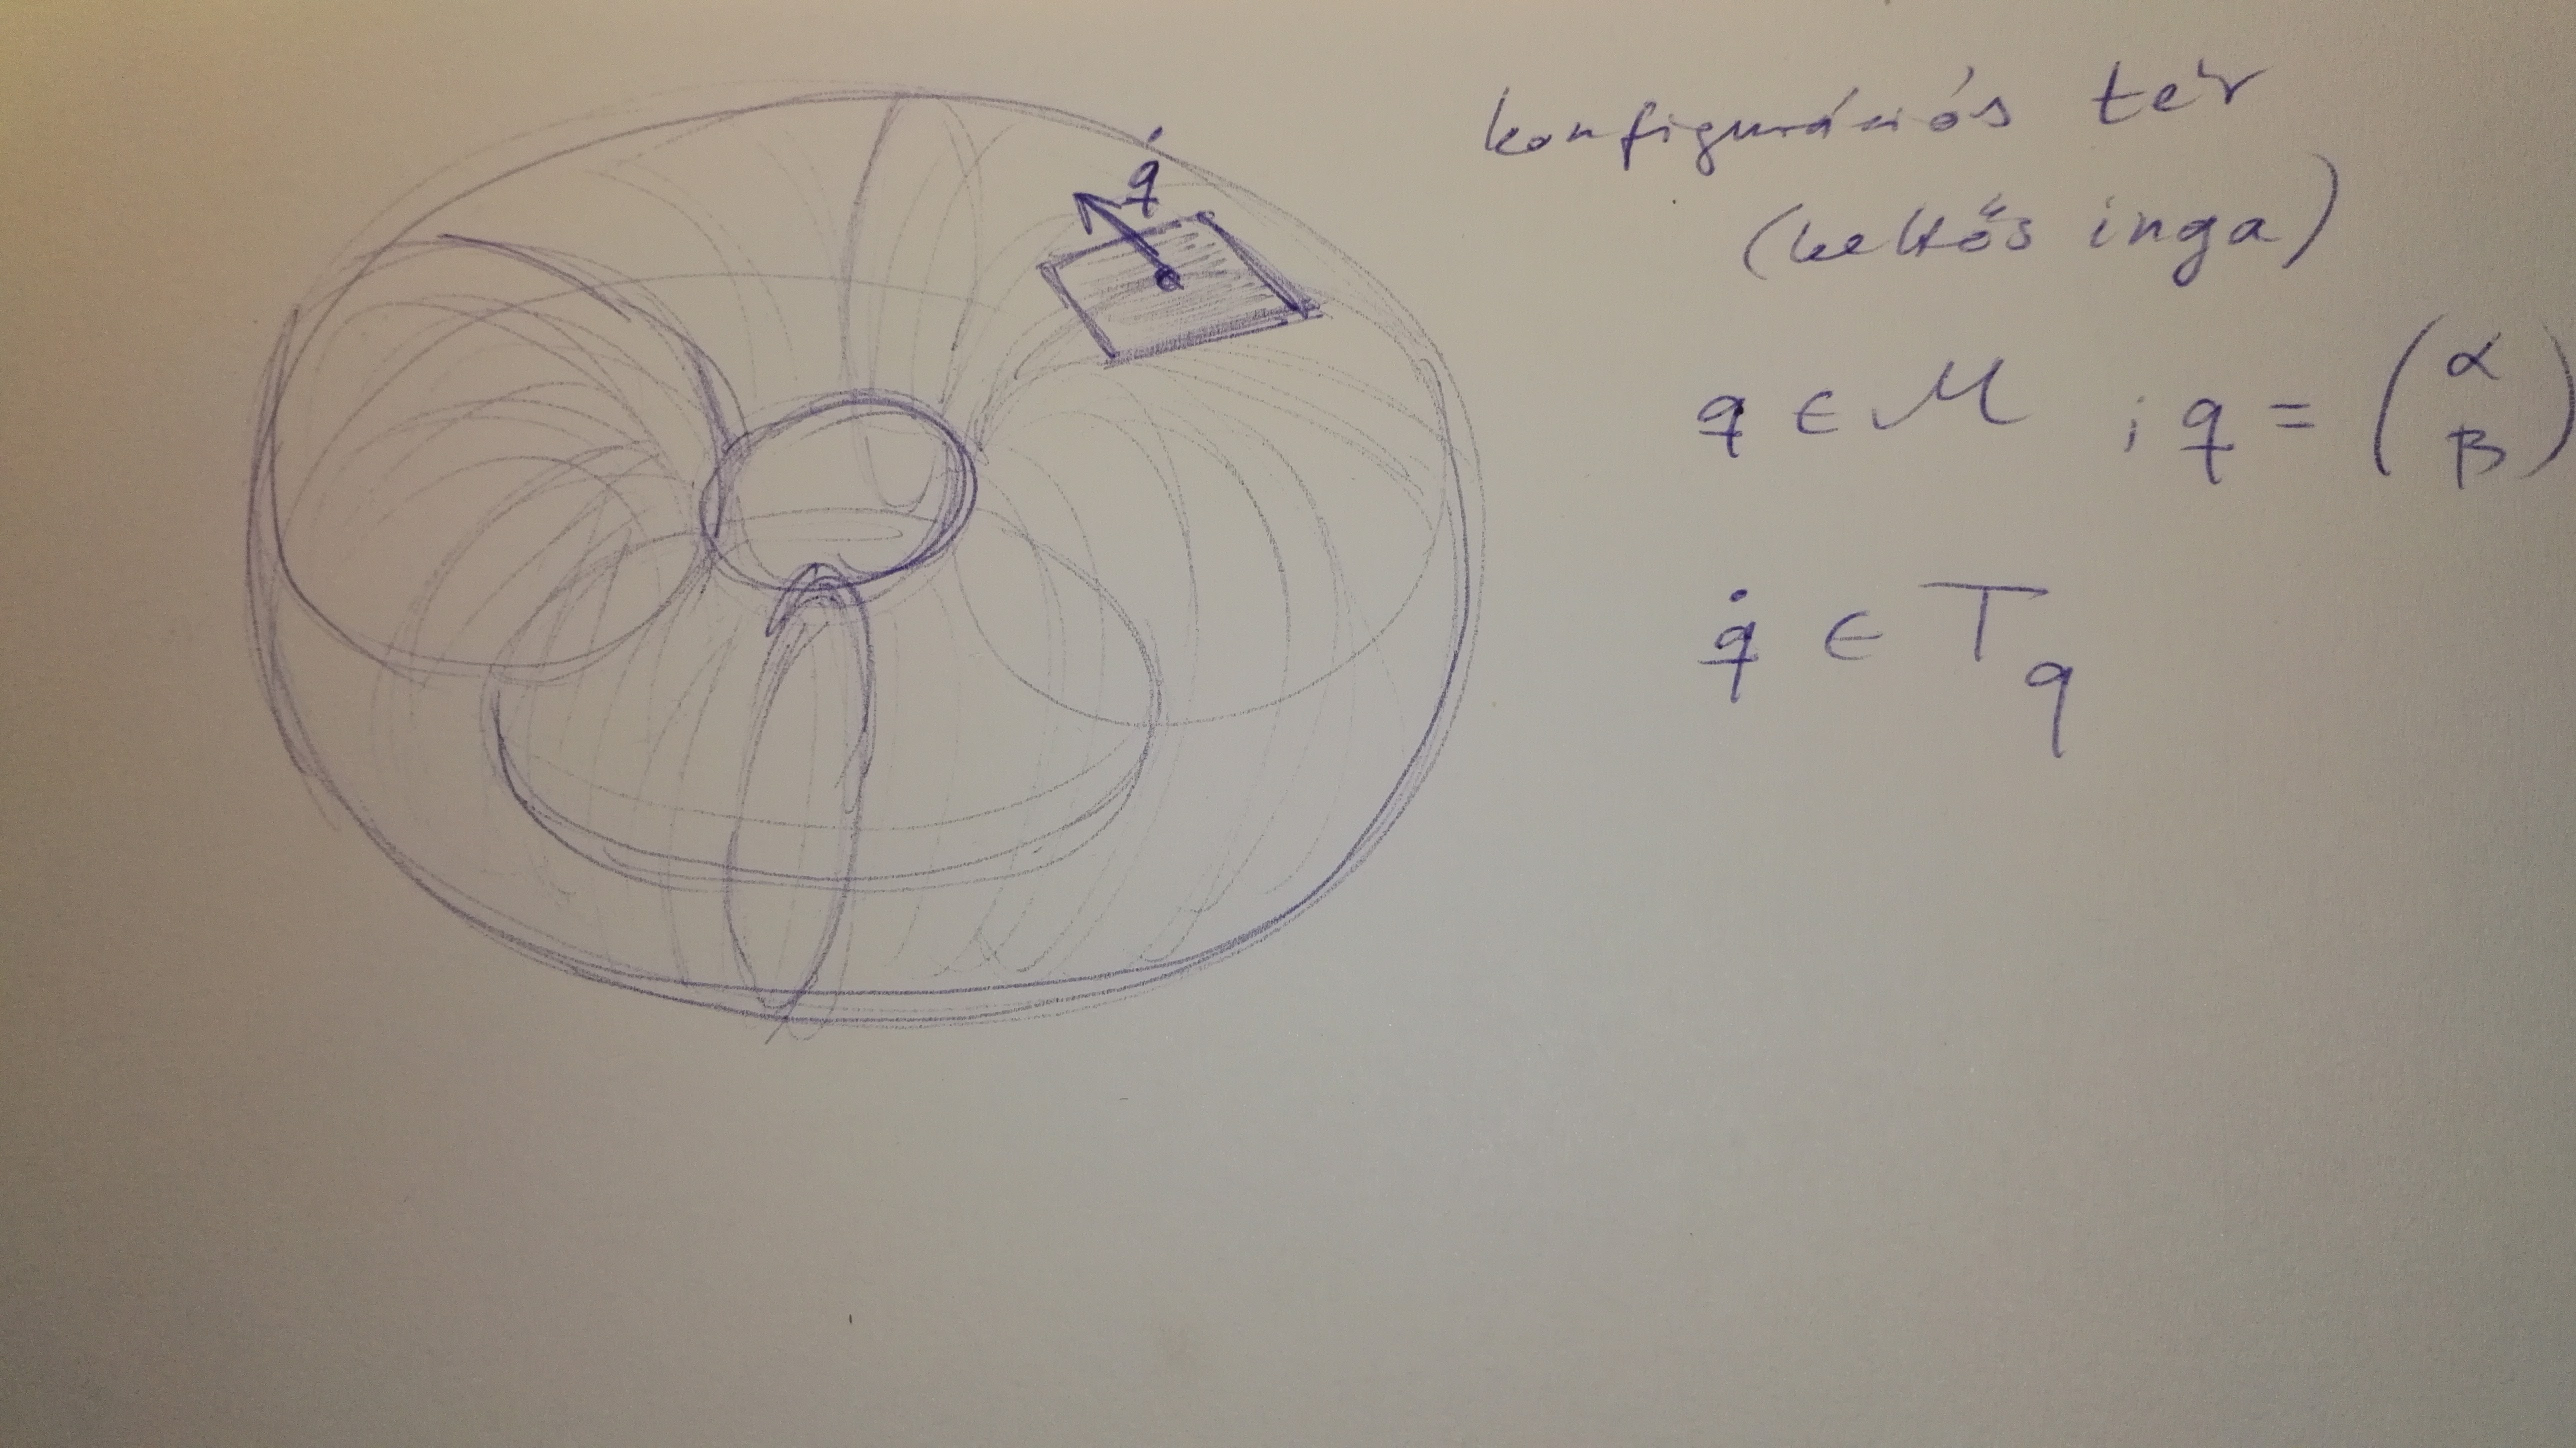
\includegraphics[width=0.9\linewidth]{konfi.jpg}
\caption{Konfigurációs tér}
\end{minipage}
\end{figure}
\par Ahol az utóbbi a kettős inga konfigurációs terén értelmezett érintőtér, vagyis az általános koordináták deriváltja. Tehát lényegében a Lagrange-függvény a konfigurációs tér érintőterén értelmezett függvény.
\newline
\par A sokaság lokálisan $\textsl{homeomorf}$ $R^{n}$-el. Azaz kölcsönösen egyértelműen és folytonos leképezhető, persze csak akkor ha $n$ véges. A sokaság olyan topologikus tér, amely mindenhol lokálisan homeomorf $R^{n}$-el. Topologikus struktúránk tehát már van, de távolság fogalom még mindig nincs a sokaságon értelmezve.
\subsection{ Duális terek fogalma}
\par Legyenek ($V_S$,+,$\cdot$), valamint ($W_S$,+,$\cdot$) vektorterek ugyanazon skalártest felett és $\textsl{A} : V \rightarrow W$ lineáris leképezés. Ezeken értelmezett az összeadás és a számmal szorzás így lineráis teret alkotnak az operátorok is.  Mi most egy speciális esetet vizsgálunk, amikor is $W_S = S$, mivel ekkor a lineáris leképezéseink funkcionálok, vagyis egy vektortérből skalárhalmazba képező függvények (lineritás továbbra is fennáll természetesen).
\par A továbbiakban $S$ megegyezik a valós számok halmazával. Mostantól pedig a teret, amelyben a funkcionáljaink laknak hívjuk a $V$-hez tartozó $V^{*}$ duális térnek, vagy röviden $V$ duálisának. A funkcionálok lineáris teret alkotnak:
\begin{itemize}
\item $\varphi, \psi \in V^{*}$, valamint $x \in V$ és $\alpha \in R$:
\item $(\varphi + \psi)x = \varphi x + \psi x$
\item $(\alpha \varphi)x = \alpha (\varphi x)$
\end{itemize}
\par Ahhoz, hogy erről a duális térről megállapítsuk, hogy hány dimenziós válasszunk benne egy bázist. Legyenek $\{\vec{e}_{k}\}_{k = 1}^{n}$ $\in$ $V$. Bármelyik $\vec{a} \in V$ előáll ezek lineárkombinációjaként. Ekkor:
\begin{align*}
\varphi\vec{a} = \varphi(a^{k}\vec{e}_{k}) = a^{k}\varphi\vec{e}_{k} \quad  \quad a^{k} \in R \\
\varphi\vec{e}_{k} = \varphi_{k} \in R
\end{align*}
tehát a funcionált is n darab adattal tudjuk reprezentálni. Bevezetve speciális $\epsilon^{k} \in V^{*}$ olyan, hogy $\epsilon^{k}\vec{e}_{l} = \delta_{l}^{k}$. Ha előállítunk egy $\Phi \in V^{*}$ funkcionált a következő módon:
\begin{align*}
\Phi = \varphi_{k}\epsilon^{k} \in V^{*} \\
\Phi\vec{a} = \varphi_{k}\epsilon^{k}\vec{a} = \varphi_{k}a^{k} = \varphi\vec{a} \\
\rightarrow \Phi = \varphi \in V^{*}
\end{align*}
\par Vagyis ez azt jelenti, hogy véges dimenziós esetben a vektortér bázisai kölcsönösen megfeleltethetőek a duális térben $\epsilon^{k}$ bázisoknak így $dimV = dimV^{*}$ feltétel teljesül. Emelett elfogadjuk, hogy egy vektortér duálisának a duálisa a kezdeti vektortér, valamint, hogy egy vektortér és duálisa izomorfak.
\newline
\par Most, hogy már bevezettük a duális terek fogalmát vegyük észre, hogy egy adott vektorhoz a duális térből rendelt elem önkényes, valamilyen előre definiált válaszott művelet kell hozzá. Legyen $\vec{a} \in \textsl{V}$, ahol adott bázis mellett $\vec{a} = a^{k}\vec{e}_{k}$. Rendeljük ehhez a duális tér egy $b$ elemét, ahol szintén bázisválasztás után, $b = b_{k}\epsilon^{k}$. Ez a hozzárendelés önkényes, hiszen most definiáljuk, hogy legyen $b_{k} = g_{kl}a^{l}$ és ezentúl jelölésben pedig $b = a^{+}$ használunk majd. Itt $g_{kl}$ a $\textit{metrikus tenzor}$. Ezzel már értelmezhető az elemek közötti skaláris szorzás.
\subsection{ Derivációk}
\par Legyenek $\Phi, \Psi : \textsl{M} \rightarrow \textsl{R}$ skalármezők. Legyen továbbá $\sum$ az ilyen skalármezők halmaza. Ezen értelmezve van a mezők számmal szorzása, a mezők összege, és a mezők egymással való szorzása is.
\par Legyen $D : \sum \rightarrow \sum$ lineáris leképezés és legyen a neve $\textsl{DERIVÁCIÓ}$. A művelet szamábalyi a követekező képpen fogalmazhatóak meg:
\begin{itemize}
\item $D(\alpha\Phi + \beta\Psi) = \alpha(D\Phi) + \beta(D\Psi)$
\item $D(\Phi\Psi) = (D\Phi)\Psi + \Phi(D\Psi)$
\end{itemize}
\par A derivációk vektorteret alkotnak. Lévén, hogy $\alpha D_1 + \beta D_2$ is deriváció.
\newline
\par Hogyan is lehet ezeket elképzelni? Először is, olyan művelet kell, ami skalármezőből, skalármezőt csinál. Lineárisnak kell lennie és vektorteret kell alkosson. Ki kell elégítenie a megadott követelményeket is. Vegyük észre, hogy nem véletlen a név, hiszen a fentebbi szabályok is valami féle deriválásra utalnak. Jó példa lehet a deriváció műveletére a $\underline{v}\hspace{0.1cm}\underline{\nabla}$ operáció. 
\par Vizsgáljuk egy adott pontban az ott átmenő összes görbét., legyenek ezek $\underline{r}_{1}(t_1), \underline{r}_{2}(t_2)$. Ezeket úgy paraméterezzük, hogy $t = 0$ időpillanatban legyen az összes $\underline{R}$. Minden pontban értelmezve van $\dot{\underline{r}}_{k}(t)$ és adott pontban lineáris teret alkot ezek összessége. Adott pontban tehát $\dot{\underline{r}}_{k}(t_k)\nabla$ operáció deriváció. A probléma csupán az, hogy ez nagyon szemléletesen definiálható $\textsl{R}^{n}$-ben, de nekünk most ugyan ez kéne a sokaságon. Ismét ahhoz folyamodunk, hogy az absztrakt halmazon úgy definiáljuk ezeket, hogy az a térképezéseknek és paraméterezéseknek eleget tegyen. 
%%% Ezt a részt annyira nem értem. Át kéne beszélnem a többiekkel, meg jó lenne ha fenn lennének már a videók...
\par Így bevezethetünk egy:
\begin{equation*}
    \Psi = v^{k}\partial_{k}\Phi = \dot{r}^{k}\partial_{k}\Phi = \frac{dx^{k}}{dt}\partial_k\Phi \quad \quad \rightarrow \frac{dx^{k}}{dt}\partial_{k}
\end{equation*}
\par Ahol $\frac{dx^{k}}{dt}\partial_{k}$ mennyiségben $\partial_{k}$ bázis vektorhoz hasonlít és az is. Adott pontban ezek feszítenek ki egy lineáris teret. Ezt nevezzük a sokaság adott pontbeli érintő terének. Lényegében a $\partial_{k}$-k az adott pontbeli vektortér bázis vektorai. Ez szemléletesen azt jelenti, hogy ha egy változót kiválasztunk, akkor az aszerint vett parciális derivált a sokaságon kijelöl görbéket, amelyeket azon változó változtatása mellett a többit állandóan tartva kaptunk. Adott pontban az összes deriváció előállítható a deriválások lineáris kombinációjaként.
\begin{figure}[H]
\centering
\begin{minipage}{0.46\linewidth}
\centering
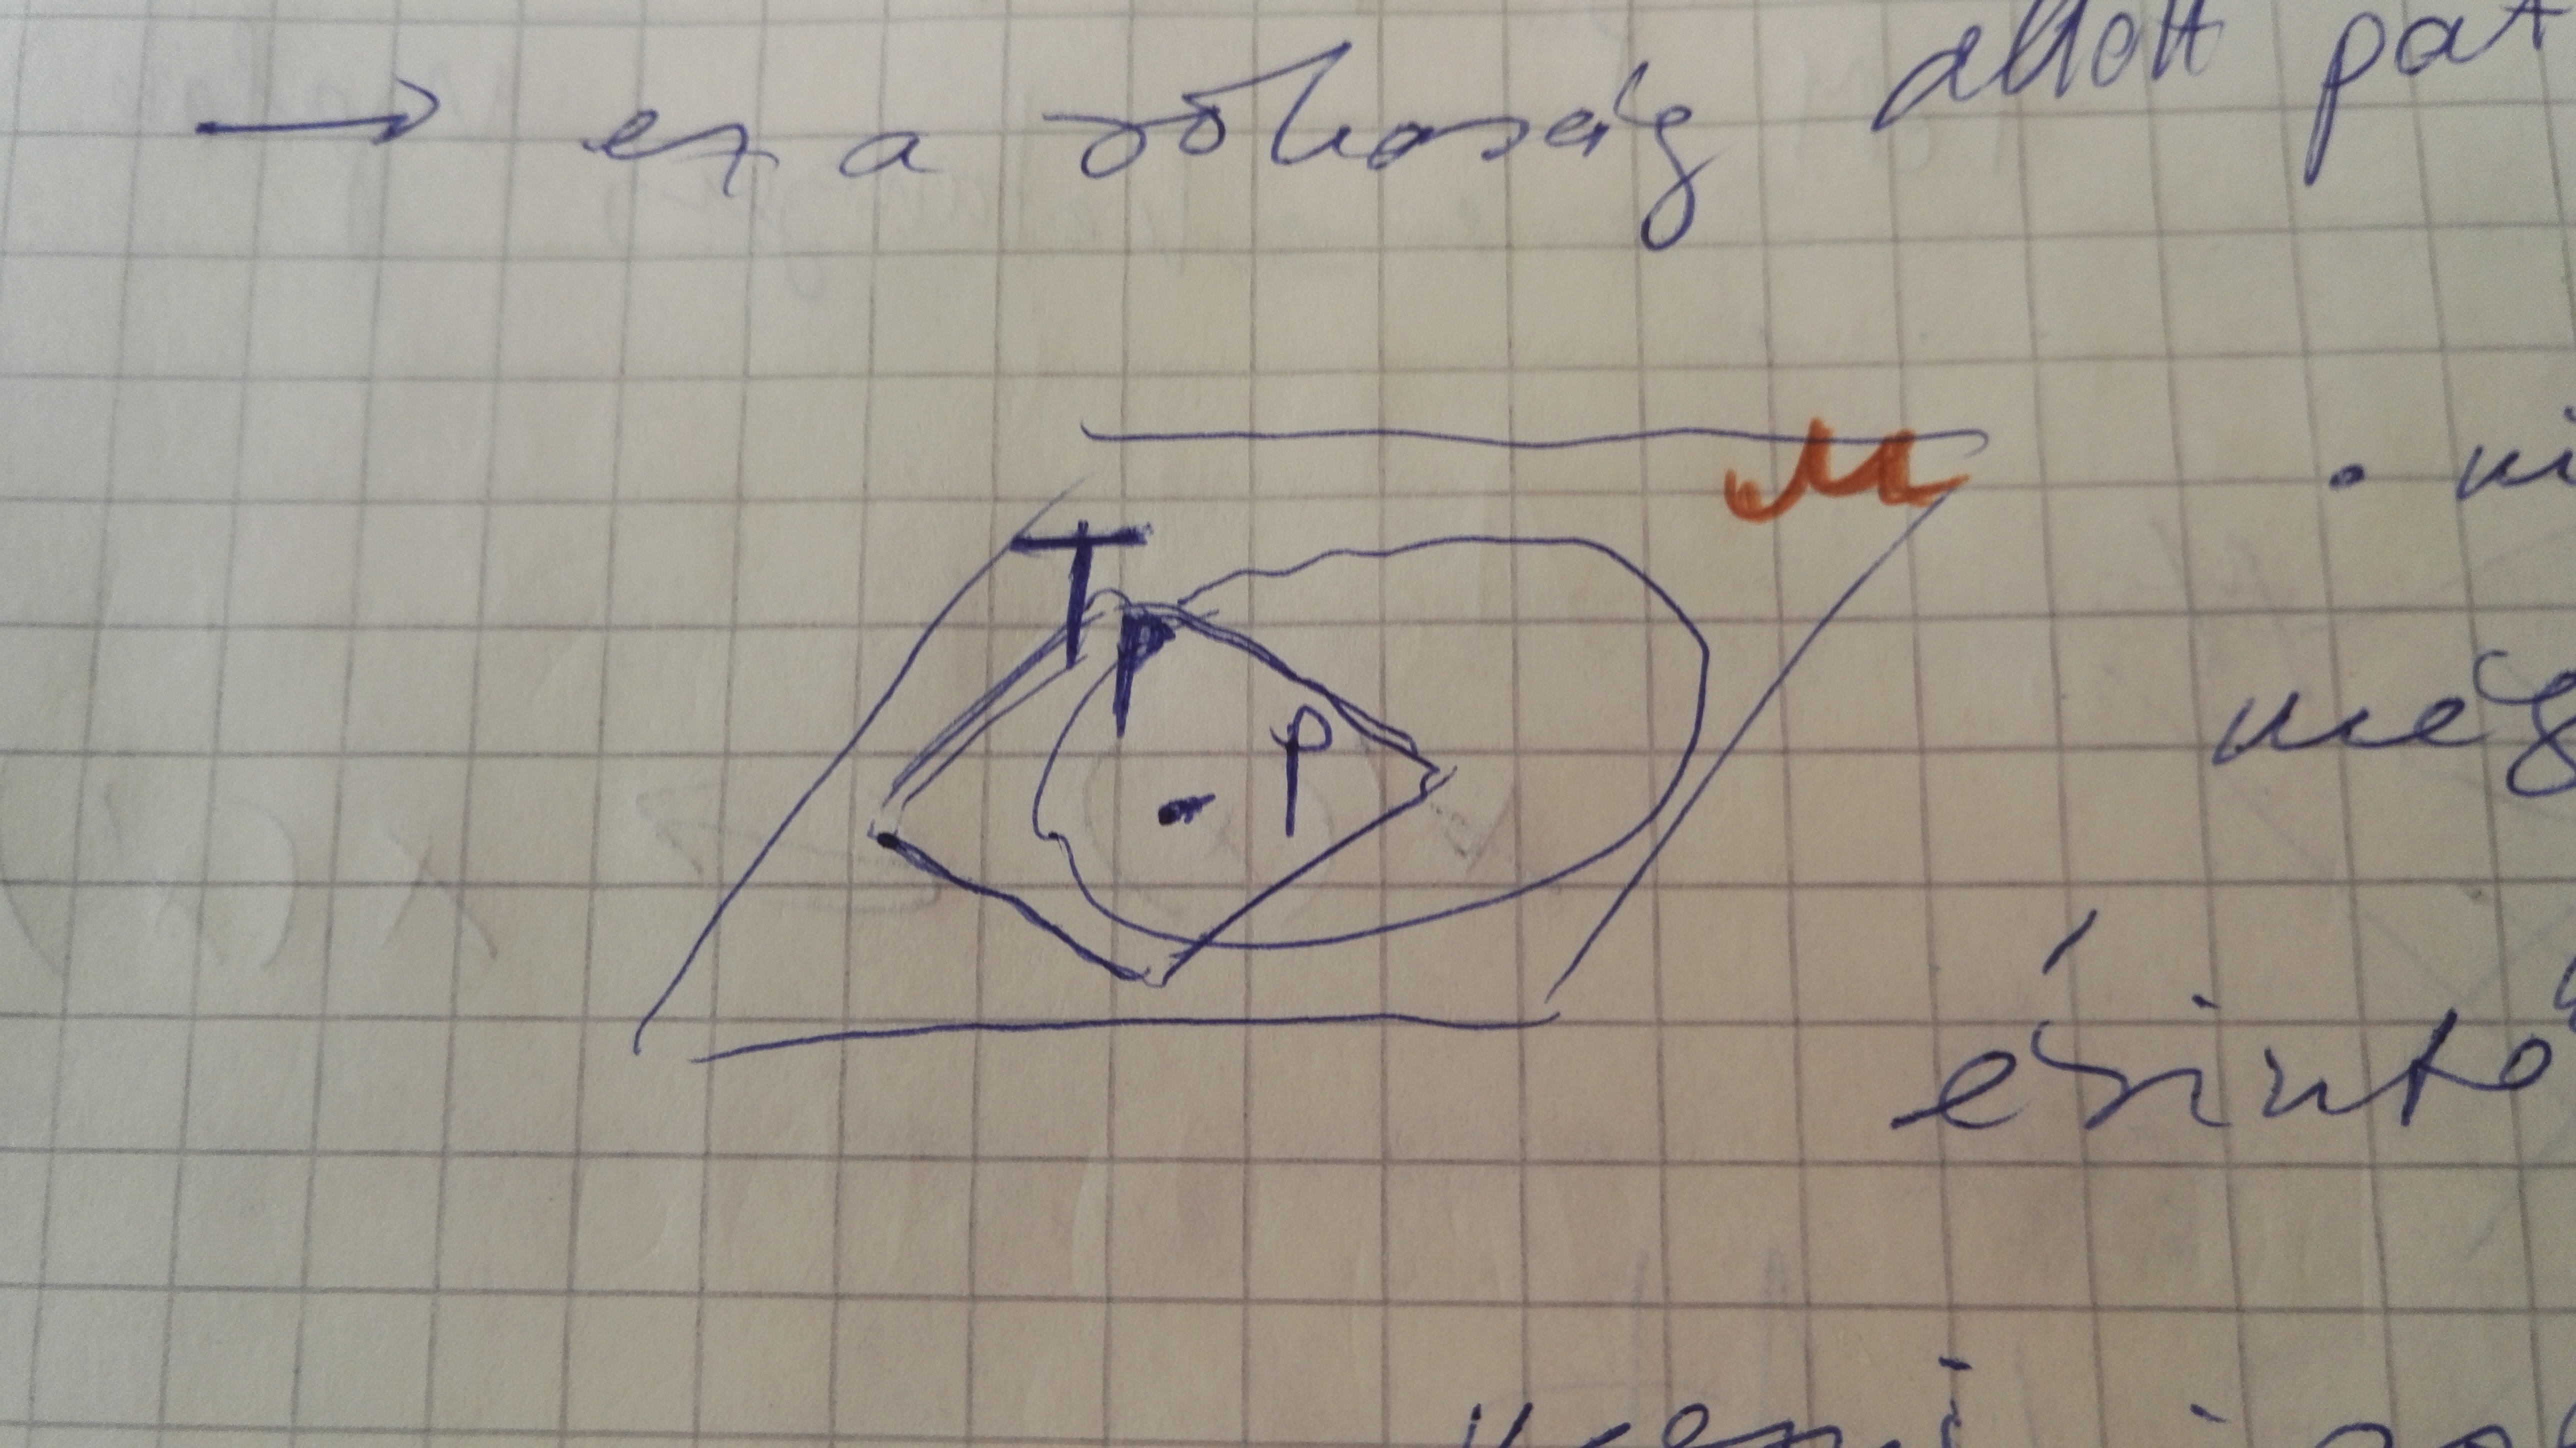
\includegraphics[width=0.9\linewidth]{erintoter.jpg}
\caption{Érintőtér}
\end{minipage}
\begin{minipage}{0.46\linewidth}
\centering
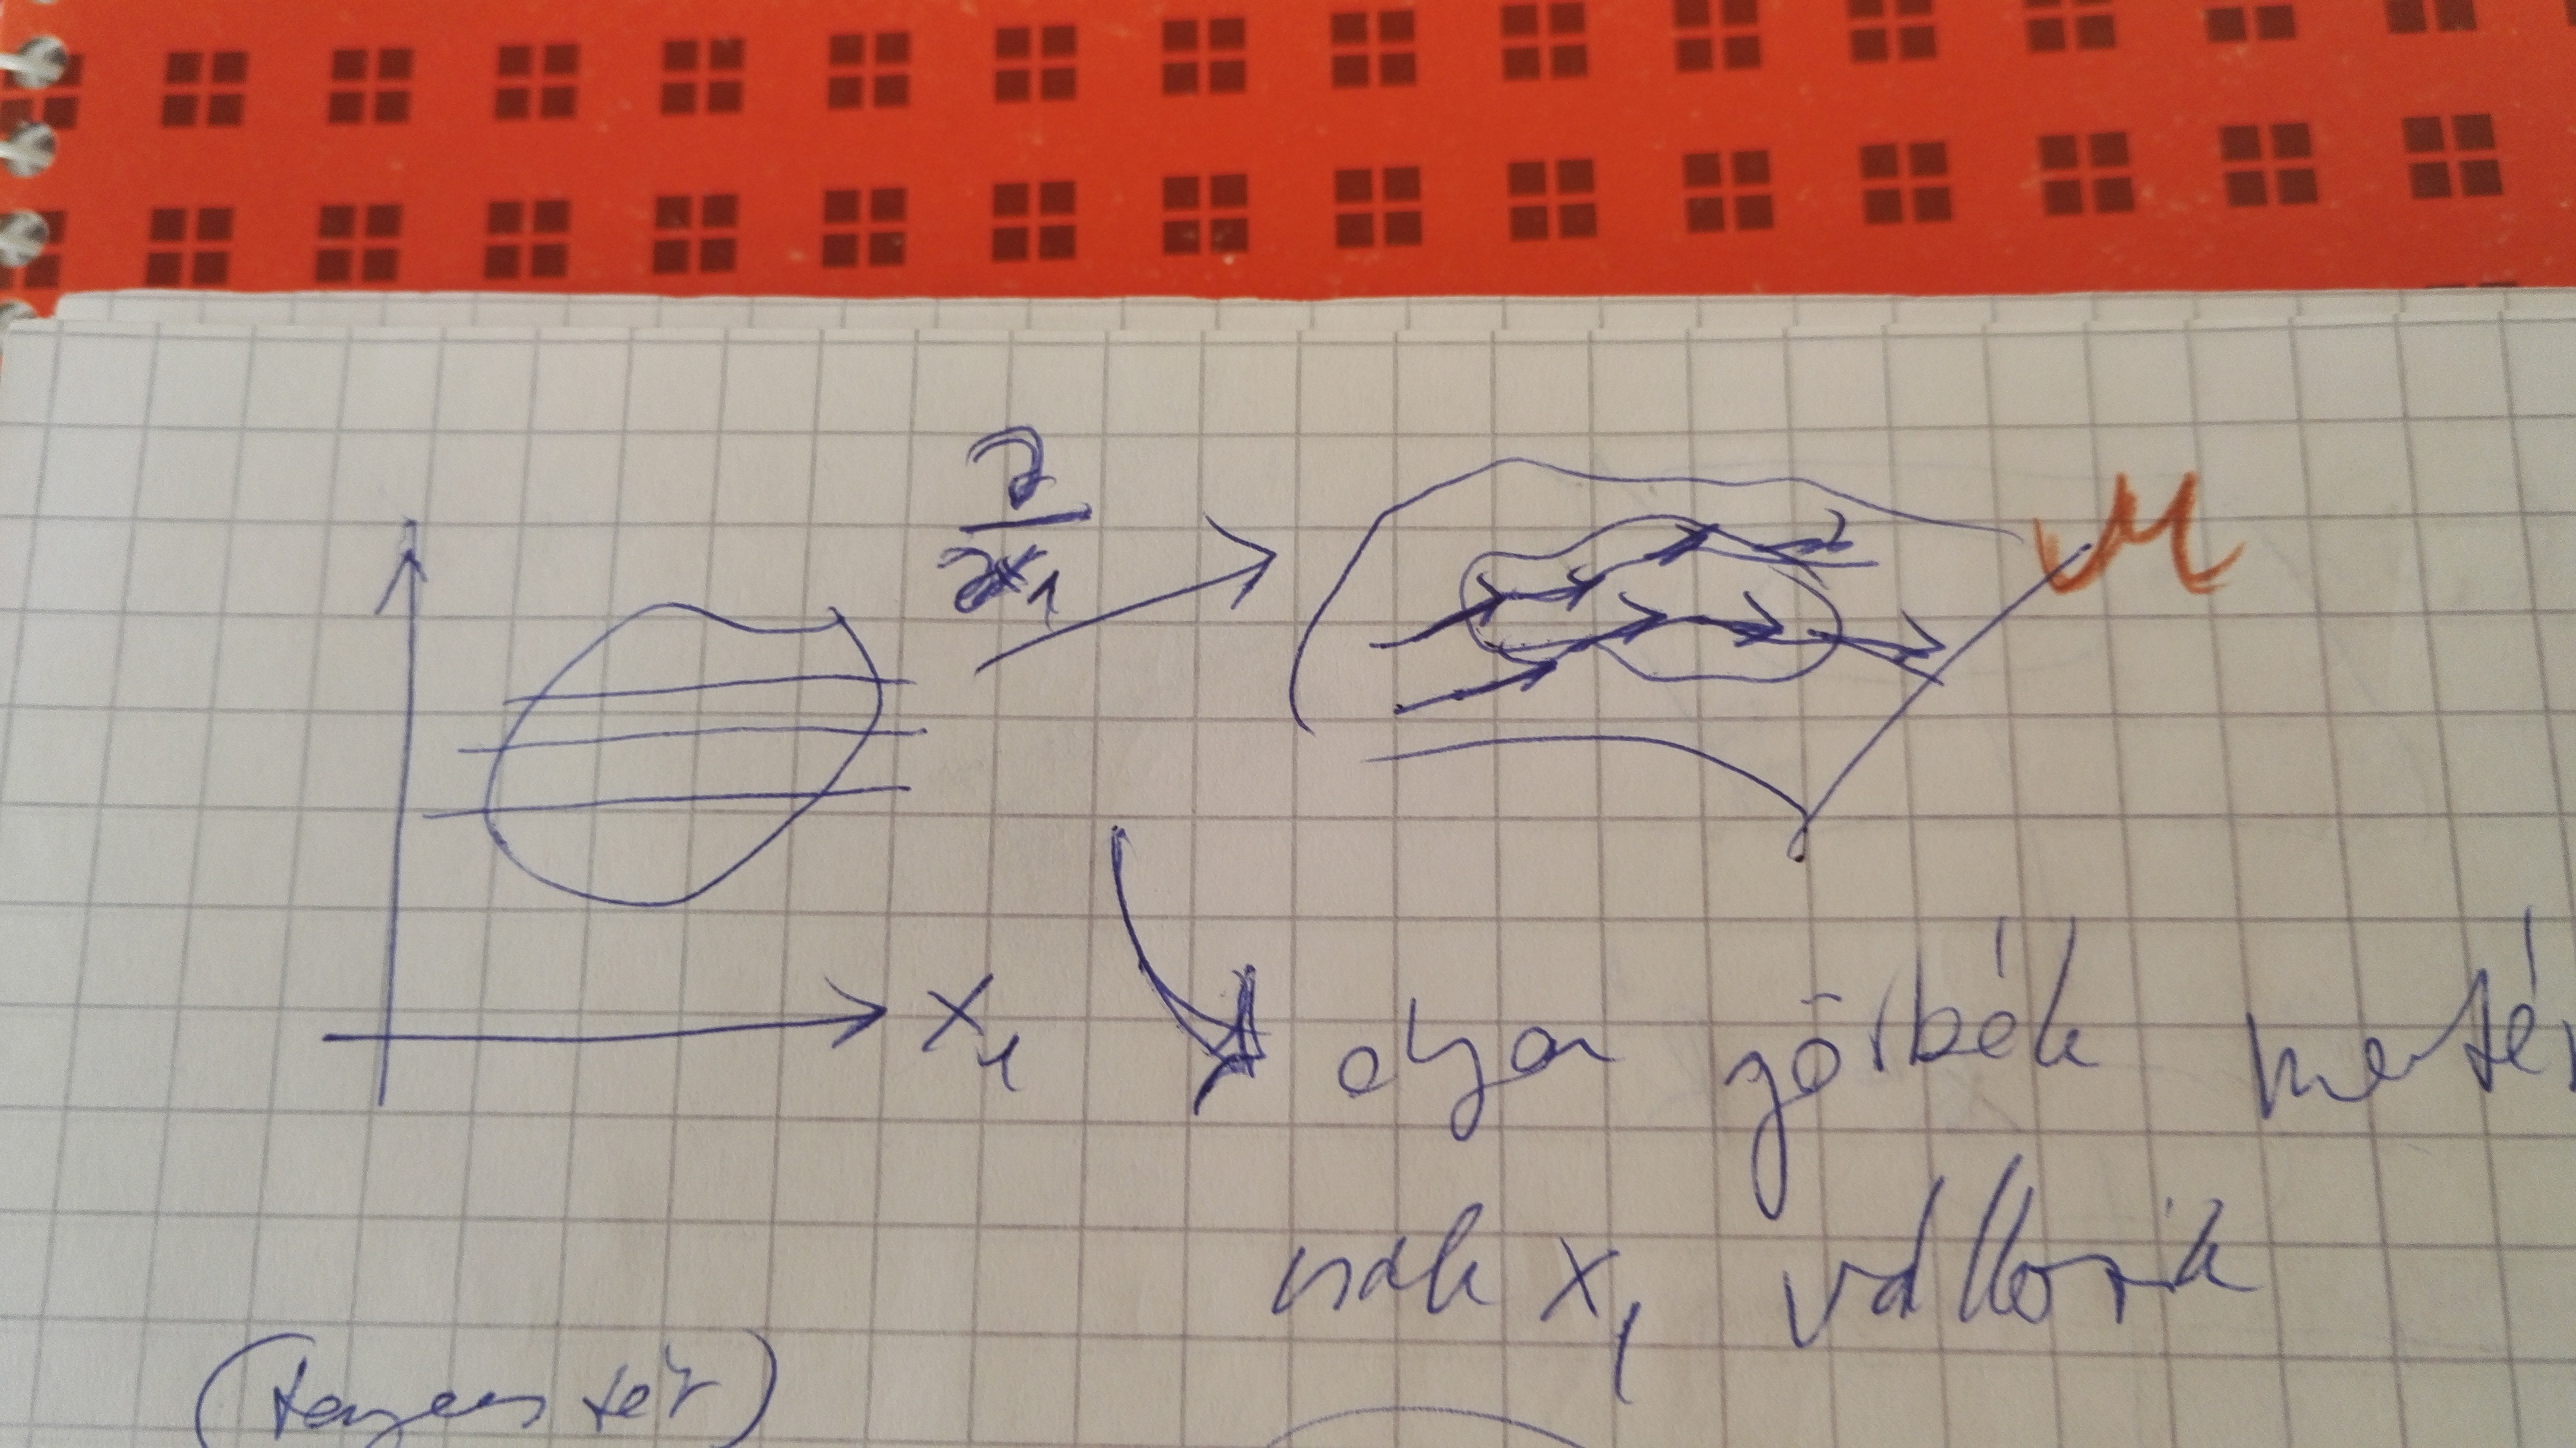
\includegraphics[width=0.9\linewidth]{derivacio.jpg}
\caption{Parciális deriváltak, mint bázisvektorok}
\end{minipage}
\end{figure}
\par Ezeket a $\partial_{k}$-kat úgy lehet szemléletesen elképzelni, hogy olyan görbéket határoz meg a sokaságon, amelyek paraméterezésének csak a k. koordinátája változik. Így a sokaság tangens nyalábját:
\begin{equation*}
    \cup_{P\in M}^{}T_{P}
\end{equation*}
\par Ha készítünk kétféle paraméterezést a sokaság adott pontjában, akkor ezek között kölcsönösen egyértelmű leképezés van. A két leképezésen véve a szintvonalakat azok őse a sokaságon kijelöl görbéket. Ezen görbék mentén vett bázis vektorokkal fel lehet írni egy derivációt, mint a $\partial_{k}$-k lineáris kombinációját, hiszen ezek mind $T_{P}$-ben vannak. Tehát véve az egyik leképezésen egy skalármezőt $\Phi(x^{k})$ és erre hattatva az előbbi derivációt a következőt:
\begin{equation*}
    D\Phi = v^{k}\frac{\partial\Phi}{\partial x^{k}}
\end{equation*}
\par Ha $\Phi(x^{k})$-t kifejezzük a másik leképezésen, akkor $\Phi(x'^{k}(x^{k}))$-n mivel kölcsönösen egyértelmű a hozzárendelés a két leképezés között, így:
\begin{equation*}
    \Psi = v^{k}\partial_{k}\Phi = v^{k}\partial_{k}(\Phi(x'(x))) = v^{k}\frac{\partial\Phi}{\partial x'^{l}}\frac{\partial x'^{l}}{\partial x^{k}}
\end{equation*}
\par Ahol a koordináták közötti két indexes mennyiséget:
\begin{equation*}
    \frac{\partial x'^{l}}{\partial x^{k}} = A^{l}_{k}(x)
\end{equation*}
\par Amivel már könnyen láthatjuk, hogy a $v^{k}$ komponensek a következőképpen transzformálódnak:
\begin{gather*}
    v'^{l} = A^{l}_{k}(x)v^{k} \\
    \Psi = v^{k}\partial_{k}\Phi = v'^{l}\partial'_{l}\Phi
\end{gather*}
\par Fontos megjegyezni, hogy $A$ egy lineáris transzformáció lokálisan, viszont globálisan hely függő, így nem tudunk globális valamilyen 'szép' leképezést adni, csak lokálisan, akkor viszont $A$ egy konstans mátrix. Ennek segítségével már kimondhatjuk, hogy vektor az ami így transzformálódik. Adott pontban már értelmezhetünk vektor mezőt. 
\par Most már tudjuk, hogy a kontra variáns (felső indexes) vektorok hogy transzformálódnak, most tehát meg kell néznünk a kovariáns (alsó indexes) trafót is.
\begin{equation*}
    u_{k}' = \frac{\partial\Phi(x(x'))}{\partial x'^{k}} = \frac{\partial\Phi}{\partial x^{l}}\frac{\partial x^{l}}{\partial x'^{k}} = B_{k}^{l}(x')u_{l}
\end{equation*}
\par $B$ szintén lokálisan lineáris trafó globálisan pedig valami 'csúnya' transzformáció, azaz nem linearizálható. Könnyen belátható, hogy $A,B$ egymás inverzei.
\begin{gather*}
    \frac{\partial x^{k}}{\partial x^{m}} = \delta^{k}_{m} \\
    \frac{\partial x^{k}}{\partial x^{m}} = \frac{\partial x^{k}}{\partial x'^{l}}\frac{\partial x'^{l}}{\partial x^{m}} = \\
    A^{k}_{l}B^{l}_{m} = \delta^{k}_{m}
\end{gather*}
\par Miután vektorok trafóját értelmeztük, értelmezhető a tenzor fogalom is. Hiszen tenzor az, ami úgy transzformálódik, mint vektor komponensek szorzata:
\begin{gather*}
    T^{kl\prime} = A^{k}_{p}A^{l}_{q}T^{pq} \\
    T'_{kl} = B_{k}^{p}B_{l}^{q}T_{pq} \\
    T^{kl}_{m\prime} = A^{k}_{p} A^{l}_{q} B^{r}_{m} T^{pq}_{r}
\end{gather*}
\par Még mindig nem jutottunk el a Riemann-geometriáig, mivel nincs metrikus tenzorunk, nincs még távolság fogalmunk. Kell egy metrikus-tenzor!
\section{ Riemann-geometria, metrikus-tenzor}
\par Legyen a sokaság P pontjában $T_{P}$ lineáris érintő tér és $T^{*}_{P}$ az ehhez tartozó kotangens tér. A duális térbeli bázis szimbólumok pedig a $dx^{k}$-k lesznek. Így a potenciál megváltozása:
\begin{equation*}
    d\Phi = \partial_k \Phi dx^{k}
\end{equation*}
\par Legyen most metrikánk. Legyen $V$ vektortér és $V^{*}$ ennek duális tere. Ezekben legyenek bázisaink és egy egymásra képző műveletünk. 
\begin{align*}
    v^{k}e_{(k)} \in V \\
    u_{l}f^{(l)} \in V^{*} \\ \\
    v_{k} = g_{kl}v^{l} \quad \quad g : V \rightarrow V^{*} \\
    v^{l} = G^{lm}v_{m} \quad \quad G : V \rightarrow V^{*} \\ \\
    G = g^{-1}
\end{align*}
\par Viszont lineáris műveletet csak mezőként, itt tenzor mezőként lehet értelmezni. Tehát $g_{kl}(x)$ leképezés minden pontban értelmezett. Fizikusok között elterjedt, hogy a $g$ leképezés inverzét is $g$-vel jelölik, azaz nem különböztetik meg a terek közötti leképezéseket betűvel csak indexeikben. Legyen tehát:
\begin{equation*}
    G^{kl}(x) = g^{kl}(x) = B^{k}_{q}(x)B^{l}_{p}(x)g_{qp}(x)
\end{equation*}
\par A metrikus tenzor bevezetése teljesen önkényes. Riemann azt követelte meg, hogy $g$ legyen pozitív definit mátrix így két pont közötti távolságot mindig pozitívnak tudott definiálni. Az általános relativitáselméletben ezt elvetjük. Az pszeudo-Riemann geometriát használ, hogy megtarthassuk a térszerű, időszerű és fényszerű 'távolságokat'. Kicsiben, azaz lokálisan vissza kell kapjuk a Minkowski-teret. Ha a metrikus tenzorral definiált skalár szorzás szimmetrikus, akkor a metrikus tenzor is az.
\begin{gather*}
    u,v \in V \\
    u^{+} \in V^{*} \\ \\
    u^{+}(v) = u_{k}v^{k} = g_{kl}u^{l}v^{k}
\end{gather*}
\par Az relativitáselméletben megköveteljük, hogy a metrikus tenzor szignatúrája (1 pozitív, 3 negatív sajátérték) megmaradjon bázistranszformáció során. Ez kell az időszerű, térszerű és fényszerű távolságok bevezetéséhez. Ez a tulajdonság csak a koordinátázástól függ. 
\par Kis elmozdulásokra a sokaságon azon pont érintő tere ahonnan az elmozdulást indítottuk közel azonosnak tekinthető a metrikus térrel. Így:
\begin{equation*}
    g_{kl}dx^{k}dx^{l} = ds^{2}
\end{equation*}
\par ívelemnégyzet definiálható. Ha $g_{kl}$ pozitív definit, akkor $\int ds$-nek mindig van értelme. Az áltrelben viszont két tetszőleges pont távolságát nem lehet értelmezni.
\par Vegyünk $R^{n}$-ben egy $w$ paraméterrel paraméterezett görbét, majd ezt 'felvetítjük' a sokaságra. Így:
\begin{gather*}
    dx^{k} = \dot{x}^{k}dw \\
    ds^{2} = g_{kl}(x(w))\dot{x}^{k}(w)\dot{x}^{l}(w)dw^{2} \\
    ds = \sqrt{g_{kl}(x(w))\dot{x}^{k}(w)\dot{x}^{l}(w)}dw \\ \\
    S = \int ds = \int_{w_{1}}^{w_{2}}f(w)dw
\end{gather*}
\par Két távoli pont távolsága csak Riemann-geometriában van értelmezve. Ennek a hatás integrálnak kell a minimumát keresni variáció számítással ($\delta S = 0$). A legutolsó képletből származtatható $Euler-Lagrange-egyenletek$kel meg lehet mondani a minimális távolságot. Az általános relativitáselméletben ahhoz, hogy két távoli pont távolságát értelmezni tudjuk más módszert kell alkalmazni.
\par Vegyünk a számunkra 'most-síkokat' a térben. Lényegében megvizsgáljuk, hogy más hely lévő megfigyelőknek hogy telik az idejük, ha nekünk $dt$ idő telik el. Tegyük fel, hogy barátainkkal együtt egy helyben állunk a tér különböző pontjaiban. Ekkor az egyén négyes vektora:
\begin{gather*}
   x^{k} = \Spvek{ct, x, y, z}
\end{gather*}
\par Ennek megváltozása szimplán az első koordinátám megváltozásából áll majd, mivel egy helyben állok, tehát $dx^{k} = cdt$. Az egy helyben állásnak van fizikai jelentése, így érdemes vizsgálni, hogy mi ennek a feltétele matematikailag. Ahhoz, hogy egy helyben tudjunk állni $dt$ ideig az szükséges, hogy a tér-időbeli pontjaink időszerűen legyenek elválasztva, azaz az ívelemnégyzet pozitív legyen.
\begin{equation*}
    ds^{2} = g_{kl}dx^{k}dx^{l} = g_{00}dx^{0}dx^{0} + 0 = g_{00}c^{2}dt^{2}
\end{equation*}
\par Azaz kikötést kaptunk $g_{00}$ értékére, miszerint annak pozitívnak kell lennie, minden vonatkoztatási rendszerben, hogy lehessen egyhelyben maradás. Ez indokolja, hogy az általános relativitáselméletben megköveteljük, hogy a metrikus tenzor szignatúra tartó legyen.
\begin{gather*}
    d\tau = \frac{1}{c}ds \\
    d\tau = \frac{1}{c}\sqrt{g_{00}c^{2}dt^{2}} \\
    d\tau = \sqrt{g_{00}(x)}dt
\end{gather*}
\par Megkaptuk tehát, hogy a sajátidő helytől függően máshogy telik az én rendszeremhez képest. A specrelben eddig ehhez arra volt szükség, hogy $Lorentz-boost$al átlépjünk egy másik rendszerbe. Itt ez a tér tulajdonsága.
\section{ Metrikus tenzor a fizikában}
\par Az elmélet kiköti, hogy nem értelmezhető tenzor, csak tenzor mező. Ezek közül kitüntetünk egyet és az lesz a metrikus tenzor. Bizonyos tulajdonságokat előírunk, hogy a végén valamilyen értelmes fizikát kapjunk az egészből. Fizikus módi, hogy a metrikus tenzor inverzét ugyan azzal a betűvel jelöljük, mint magát a tenzort. 
\par Einstein elvetette a metrikus tenzor pozitív definitségét így nem értelmezhető távoli pontok távolsága. 
\par Orientálható sokaságokkal foglalkozunk. Erre pontos definíciót nem adunk. A szemléletes magyarázat az, hogy ha kiválasztunk egy jövőbe mutató vektort akkor azt nem lehet addig transzformálni, míg valamilyen rendszerben múltba tartó nem lesz. A metrikus tenzort úgy kell bevezetnünk, hogy ne legyen értelme a térszerű trajektóriának és egy világ vonal minden pontjába húzott érintő  jövőbe mutatónak kell legyen. 
\par A téridő koordinátázása önkényes, így nem kell, hogy $x_0$ koordináta időszerű legyen, sőt egyáltalán nincs szükség tisztán időszerű koordinátára. Így általában nincs konkrét jelentése kizárólag egy koordináta megváltozásának.
\par Vizsgáljuk a következő szituációt. Az űrben lebegünk két űrhajóval és megpróbáljuk szinkronizálni az óráinkat, hogy tudjuk mikor kell lecsapni az ellenségre. Ehhez mi fény jelet küldünk az űrhajóra, majd amint az megkapja vissza is küldi nekünk. Miután megkapjuk az üzenetet előre állítjuk az óránkat a küldés és fogadás között, számunkra eltelt idő felével, hiszen az űrhajó állandó távolságra volt tőlünk, így az újonnan szerzett időnket tekinthetjük az űrhajó $most$jának. Most pedig számoljunk, szem előtt tartva, hogy a fény terjedése során az ívelemnégyzet mindig zérus.
\begin{gather*}
    ds^{2} = g_{kl}dx^{k}dx^{l} = g_{00}dx^{0}dx^{0} + g_{0\alpha}dx^{0}dx^{\alpha} + g_{\alpha 0}dx^{0}dx^{\alpha} +
    g_{\alpha\beta}dx^{\alpha}dx^{\beta} = 0 \\
    dx^{\alpha} = konstans \\
    ds^{2} = g_{00}(dx^{0})^{2} + 2(g_{0\alpha}dx^{\alpha})dx^{0} + (g_{\alpha\beta} dx^{\alpha}dx^{\beta}) = 0
\end{gather*}
\par A másodfokú egyenlet két megoldása pontosan megadja a jel megkapásától indított fény kúp és a küldő űrhajó idő vonalának két metszés pontját, azaz a küldési és fogadási időpontokat. Ezek átlaga a Vi\`ete-formulákat alkalmazva:
\begin{equation}
    dx^{0}_{new} = \frac{dx_{1}^{0} + dx_2^{0}}{2} = -\frac{g_{0\alpha}}{g_{00}}dx^{\alpha}
\end{equation}
\par Viszont van egy aprócska probléma. Ez csak szomszédok között működik! Sajnos nem lehet egy egész flottát szinkronizálni. Csak akkor lenne lehetséges, ha $g_{0\alpha} = 0$ lenne. Adott rendszerben mindig tudunk olyan metrikus tenzort konstruálni, ami ilyen, így a szinkronizálhatóság definiálható, de ez a koordinátázás tulajdonsága. Matematikailag a metrikus tenzor önkényes. Fizikailag viszont a szinkronizációból azt kapjuk, hogy valahol a múltban (Nagy Bumm) vagy a jövőben  (Nagy Reccs) szingularitást kapok. Az $Einstein-egyenletek$ből majd ez következik, de egyenlőre ez csak egy érdekes megjegyzés.
\par Most nézzük meg, hogy mit gondolunk a jelek küldési és érkezési ideje közötti különbségből milyen távolságra lehet a szomszéd űrhajó. A kezdeti most rendszerből eltelt idő:
\begin{gather*}
    \Delta t = t_{2} - t_{1} = \frac{x^{0}_{2} - x^{0}_{1}}{c}
\end{gather*}
\par Számunkra azonban a saját időnk telik az űrhajónkon, így:
\begin{gather*}
    \Delta \tau = \sqrt{g_{00}}\frac{x^{0}_{2} - x^{0}_{1}}{c}
\end{gather*}
\par Felhasználva, hogy a két koordináta különbsége éppen a korábban kiszámolt $dx_{1,2}^{0}$-k különbsége:
\begin{gather*}
    \Delta \tau = \frac{2}{c}\frac{\sqrt{(g_{0\alpha}dx^{\alpha})(g_{0\beta}dx^{\beta})-(g_{00}g_{\alpha\beta}dx^{\alpha}dx^{\beta})}}{\sqrt{g_{00}}}
\end{gather*}
\par Mivel a fény oda-vissza ugyan akkora utat tesz meg a tér időben, így $c\Delta\tau = 2\Delta l$, így:
\begin{gather*}
    \Delta l^{2} = \frac{(g_{0\alpha}dx^{\alpha})(g_{0\beta}dx^{\beta})-(g_{00}g_{\alpha\beta}dx^{\alpha}dx^{\beta})}{g_{00}} \\ \\
    \Delta l^{2} = \gamma_{\alpha\beta}(x)dx^{\alpha}dx^{\beta}
\end{gather*}
\par Ahol az utóbbi képlet szinkronizált esetben igaz, mivel akkor $g_{0\alpha} = 0$. Viszont jól látható, hogy $\gamma$ függ a rendszer időtől, azaz a távolság a két ÁLLÓ űrhajó között időben VÁLTOZIK (ld. később: a tér tágul).
\section{ Parallel transzport (párhuzamos eltolás)}
\par Tegyük fel, hogy nem létezik metrikánk, de már definiáltunk skalármezőket és szeléssel vektor mezőket is a sokaságon. Legyenek a sokaságon $P$ és $Q$ pontok infinitezimális távolságra. Ezek különböző érintő terekben vannak és míg ezeket nem transzformáljuk egybe, addig nem beszélhetünk a különbségükről, nem tudunk differenciálni. Egy-egy ilyen eltolásnál az adott pontbeli vektor komponensei megváltoznak, mivel maga a sokaság változik alatta, mint pl. polárkoordináta-rendszerben hasonló esetben.
\par Elvárjuk, hogy egy eltolás esetén a koordináták csak infinitezimálisan változzanak meg infinitezimális közelségben lévő pontok esetén. 
\begin{gather*}
    \overline{v}^{k} = v^{k} + \delta v^{k}
\end{gather*}
\par Kell egy transzformáció, amely $T_{P} \rightarrow T_{Q}$ képez. Ez önkényes, mivel most elvetettük a metrikát így nincs geometriája a rendszernek. Elvárt tulajdonságai:
\begin{itemize}
    \item legyen lineáris
    \item legyen arányos a transzformált vektorral
    \item legyen lineáris $dx$-ben is
\end{itemize}
\par Így:
\begin{equation*}
    \delta v^{k} = - \Gamma_{lm}^{k}(x)v^{l}dx^{m} 
\end{equation*}
\par csak az előbbi kifejezés lehet a vektor változását kifejező általános esetben. Az itt bevezetett több indexes mennyiség (nem tenzor ld. később) neve Christoffel-szimbólum. A következőt kaptuk tehát:
\begin{gather*}
    \overline{v}^{k} = (\delta_{l}^{k} - \Gamma_{lm}^{k}dx^{m})v^{l}
\end{gather*}
\par Ezt nevezzük konnexiónak. A $\Gamma$ mennyiség önkényes, de legyen folytonos és differenciálható. Lássuk be, hogy nem tenzor:
\begin{gather*}
    v^{k\prime} = A_{l}^{k}(x) v^{l} = \frac{\partial x^{k\prime}}{\partial x^{l}}v^{l} \\
    u_{k\prime} = B_{k}^{l}(x) u_{l} = \frac{\partial x^{l}}{\partial x^{k\prime}}u_{l} 
\end{gather*}
\par Ahogy már korábban bevezettük, egyik koordinátázásról a másikra ezen transzformációkkal térhetünk át. Most vigyük át $v^{k}$-t és $\overline{v}^{k}$-t másik koordinátázásra:
\begin{gather*}
    v^{k\prime} = A^{k}_{l}(x)v^{l} \\
    \overline{v}^{k\prime} = A^{k}_{l}(x + dx)\overline{v}^{l}
\end{gather*}
\par Ahol az utóbbit kifejtve:
\begin{align*}
    \overline{v}^{k\prime} = A^{k}_{l}(x + dx)\overline{v}^{l} = \\
    = (A^{k}_{l}(x) + \frac{\partial A^{k}_{l}}{\partial x^{m}}dx^{m})\cdot(v^{l} - \Gamma_{pq}^{l}v^{p}dx^{q}) = \\
    = A^{k}_{l}(x)v^{l} - A^{k}_{l}\Gamma^{l}_{pq}v^{p}dx^{q} + \partial_{m}A^{k}_{l}dx^{m}v^{l} + O(dx^{2}) = \\
    = v^{k\prime} - A^{k}_{p}\Gamma_{lm}^{p}v^{l}dx^{m} + \partial_{m}A^{k}_{l}dx^{m}v^{l} = \\
    = v^{k\prime} - dx^{m}v^{l}\cdot( A^{k}_{p}\Gamma_{lm}^{p} - \partial_{m}A^{k}_{l} )
\end{align*}
\par Tudjuk, hogy $v^{l} = B^{l}_{p}v^{p\prime}$ és, hogy $dx^{m} = B_{s}^{m}dx^{s\prime}$. Ezeket megfelelő indexekkel helyettesítve kapjuk, hogy:
\begin{gather*}
    \overline{v}^{k\prime} = v^{k\prime} - ( A^{k}_{p}\Gamma_{qm}^{p} - \partial_{s} A^{k}_{p} )B^{q}_{l}v^{l\prime}B_{m}^{s}dx^{m\prime}
\end{gather*}
\par Ahonnan leolvashatjuk, hogy:
\begin{equation*}
    \Gamma_{lm}^{k\prime}(x) = ( A^{k}_{p}(x)\Gamma_{qm}^{p}(x) - \partial_{s}A_{q}^{k}(x) )B_{l}^{q}(x)B_{m}^{s}(x)    
\end{equation*}
\par Jól látható, hogy ez nem tenzor, csak abban az esetben, ha $\partial_{s}A^{k}_{p} = 0$ teljesül, azaz $A$ és $B$ trafók lineárisak voltak.
\par Vegyük $T^{kl} = u^{k}v^{l}$ mennyiséget és lássuk be, hogy ez tenzor.
\begin{align*}
    \overline{T}^{kl} = \overline{u}^{k}\overline{v}^{l} = \\
    = (u^{k} + \delta u^{k})\cdot(v^{l} + \delta v^{l}) = \\
    = (u^{k} - \Gamma_{mp}^{k}u^{m}dx^{p} )\cdot(v^{l} - \Gamma_{qs}^{l}u^{q}dx^{s}) = \\
    = u^{k}v^{l} - \Gamma_{mp}^{k}u^{m}v^{l}dx^{p} - u^{k}v^{q}\Gamma_{qs}^{l}dx^{s} + O(dx^{2}) = \\
    = u^{k}v^{l} - \Gamma_{pm}^{k}u^{p}v^{l}dx^{m} - u^{k}v^{p}\Gamma_{pm}^{l}dx^{m} = \\
    = T^{kl} - (\Gamma_{pm}^{k}T^{pl} + \Gamma_{pm}^{l}T^{kp})dx^{m}
\end{align*}
\par Ahol $\Gamma_{pm}^{k}T^{pl} + \Gamma_{pm}^{l}T^{kp} = \delta T^{kl}$. Belátható, hogy ez alapján több indexes mennyiségek is hasonlóan transzformálódnak. A lényeg, hogy ki kell találni egy összegző indexet minden transzformálódó indexére a mennyiségnek, és hol az egyiket, hol a másikat megtartani, hogy szemléletesebb legyen:
\begin{equation*}
    \overline{T}^{\textbf{kl}} = T^{\textbf{kl}} - (\Gamma_{\textcolor{red}{p}\textcolor{blue}{m}}^{\textbf{k}}T^{\textcolor{red}{p}\textbf{l}} + \Gamma_{\textcolor{red}{p}\textcolor{blue}{m}}^{\textbf{l}}T^{\textbf{k}\textcolor{red}{p}})dx^{\textcolor{blue}{m}}
\end{equation*}
\par Ez alapján akkor egy három indexes tenzorra:
\begin{equation*}
    \overline{T}^{\textbf{klm}} = T^{\textbf{klm}} - (\Gamma_{\textcolor{red}{p}\textcolor{blue}{s}}^{\textbf{k}}T^{\textcolor{red}{p}\textbf{lm}} + \Gamma_{\textcolor{red}{p}\textcolor{blue}{s}}^{\textbf{l}}T^{\textbf{k}\textcolor{red}{p}\textbf{m}} + \Gamma_{\textcolor{red}{p}\textcolor{blue}{s}}^{\textbf{m}}T^{\textbf{kl}\textcolor{red}{p}})dx^{\textcolor{blue}{s}}
\end{equation*}
\par És így tovább. Most azonban nézzük meg, hogy az alsó indexes vektorok, hogyan transzformálódnak. $u_{k} \in T_{P}^{*}$ és $\overline{u}_{k} \in T_{Q}^{*}$. Ekkor az előzőekhez hasonlóan egy olyan transzformáció ami lineáris a megfelelő tagokban és infinitezimális távolságban infinitezimális a vektor megváltozása egy három indexes mennyiséggel írható le általánosan. Ez $\delta u_{k} = -F^{l}_{km}(x)u_{l}dx^{m}$.
\par Ha bevezetnénk egy skaláris szorzás jellegű műveletet, akkor örülnénk, ha az skalár lenne és maradna akkor is, ha eltoljuk. Vagyis, ha $u_{k}v^{k} = \alpha$, akkor legyen $\overline{u}_{k}\overline{v}^{k} = \alpha$. Ez teljesül:
\begin{align*}
    \overline{u}_{k}\overline{v}^{k} = \\
    = (u_{k} + \delta u_{k})\cdot(v^{k} + \delta v^{k}) = \\
    = (u_{k} - F^{l}_{km}u_{l}dx^{m})\cdot(v^{k} - \Gamma_{pq}^{k}v^{p}dx^{q}) = \\
    = u_{k}v^{k} - F_{km}^{l}u_{l}v^{k}dx^{m} - \Gamma_{pq}^{k}u_{k}v^{p}dx^{q} + O(dx^{2}) = \\
    = u_{p}v^{p} - F_{km}^{l}u_{l}v^{k}dx^{m} - \Gamma_{km}^{l}u_{l}v^{k}dx^{m} = \\
    = u_{k}v^{k} - (F_{km}^{l} + \Gamma_{km}^{l})\cdot u_{l}v^{k}dx^{m} 
\end{align*}
\par Mivel azt akarjuk, hogy ez utóbbi egyezzek meg $u_{k}v^{k}$-val, a zárójeles mennyiségnek kell azonosan nullának lennie, azaz:
\begin{equation*}
    F_{km}^{l} = -\Gamma_{km}^{l}
\end{equation*}
\par Most már akármilyen index elrendezésű tenzorok trafóját felírhatjuk:
\begin{gather*}
    \overline{T}_{\textbf{kl}} = T_{\textbf{kl}} - (-\Gamma_{\textbf{k}\textcolor{blue}{m}}^{\textcolor{red}{p}}T_{\textcolor{red}{p}\textbf{l}} + -\Gamma_{\textbf{l}\textcolor{blue}{m}}^{\textcolor{red}{p}}T_{\textbf{k}\textcolor{red}{p}})dx^{\textcolor{blue}{m}} \\
    \overline{T}_{\textbf{l}}^{\textbf{k}} = T^{\textbf{k}}_{\textbf{l}} -  (\Gamma_{\textcolor{red}{p}\textcolor{blue}{m}}^{\textbf{k}}T^{\textcolor{red}{p}}_{\textbf{l}} + -\Gamma_{\textbf{l}\textcolor{blue}{m}}^{\textcolor{red}{p}}T^{\textbf{k}}_{\textcolor{red}{p}})dx^{\textcolor{blue}{m}}
\end{gather*}
\par Az infinitezimális eltolást kellő részletességgel vizsgáltuk, viszont mi van, akkor ha nem szomszédos, hanem távolabbi pontba transzformálunk? Sok kis lépésből összerakva elvileg már lehetséges $x^{k}(w)$ görbén haladni. ( $w$ paraméter ).
\begin{equation*}
    v^{k}(w+dw) = v^{k}(w) - \Gamma_{lm}^{k}(x(w))v^{l}(w)dx^{m}
\end{equation*}
\par Az kell, hogy a trafó a görbe mentén essen meg $dw$-vel, nem akárhol a sokaságon. Ekkor $dx^{m} = \dot{x}^{m}dw$ és $v^{k}(w+dw) = v^{k}(w) + \dot{v}^{k}(w)dw$, tehát:
\begin{equation*}
    \dot{v}^{k}(w) = -\Gamma_{lm}^{k}(w)v^{l}(w)\dot{x}^{m}(w)
\end{equation*}
\par Ez $v^{k}(w)$-re egy differenciál egyenlet rendszer, ami változó együtthatós és lineáris. Legyen $-\Gamma_{lm}^{k}(w)\dot{x}^{m}(w) = M^{k}_{l}(w)$, ekkor az egyenlet a következőképpen módosul:
\begin{equation*}
    \underline{\dot{v}} = \doubleunderline{M}\cdot\underline{v}
\end{equation*}
\par Megfelelő kezdő feltételekkel létezik egyértelmű megoldás.
\section{ Kovariáns derivált}
\par Görbült sokaságnak nevezünk egy sokaságot, ha egy benne zárt úton vett vektor iránya a kezdő és végpontokban nem ugyan az. (Ennél sokkal pontosabb definíciót nem adunk, elvégre ez nem analízis óra, meg senki nem is igényli.) 
\par Definiáljunk egy olyan görbét, melynek érintő vektorát eltolva az önmagába megy át, általánosan ez lenne az egyenes definíciója. Az előbb beláttuk, hogy a görbe mentén vett vektor $\dot{v}_{k}(w) = M^{k}_{l}(w)v^{l}(w)$ módon transzformálódik, most csak ugyan ezt kell alkalmaznunk $\dot{x}^{k}(w)$-ra, ami $x^{k}(w)$ görbe érintő vektora. Erre felírva az előbbi egyenletet, és $M^{k}_{l}(w)$-t kifejtve kapjuk:
\begin{equation*}
    \ddot{x}^{k}(w) = - \Gamma_{lm}^{k}(w)\dot{x}^{l}(w)\dot{x}^{m}(w)
\end{equation*}
\par Ezt átrendezve kapjuk, hogy:
\begin{equation*}
    \ddot{x}^{k}(w) + \Gamma_{lm}^{k}(w)\dot{x}^{l}(w)\dot{x}^{m}(w) = 0
\end{equation*}
\par Amit $\dot{x}^{k}(w)$ kovariáns differenciáljának nevezünk és a következő jelölést alkalmazzuk rá:
\begin{equation*}
    \frac{D \dot{x}^{k}}{dw} = 0
\end{equation*}
\par Általánosan tehát azt mondhatjuk, hogy egy $v^{k}(w)$ vektor kovariáns deriváltja a következő képpen néz ki:
\begin{gather*}
    \frac{Dv^{k}}{dw} = \frac{dv^{k}}{dw} + \Gamma_{lm}^{k}v^{l}\frac{dx^{m}}{dw} \\
    Dv^{k} = dv^{k} + \Gamma_{lm}^{k}v^{l}dx^{m}
\end{gather*}
\par Legyen most a sokaságunk minden pontjában egy vektor mezőnk. Kössük ki, hogy:
\begin{equation*}
    v^{k}(Q) - \overline{v}^{k}(P) = Dv^{k}
\end{equation*}
\par Vagyis a sokaság $Q$ pontjában vett vektorunk és a sokaság $P$ pontjából a $Q$ pontba eltolt vektorok különbsége legyen a kovariáns differencia. Továbbvive ezt a gondolatot:
\begin{align*}
    v^{k}(Q) - \overline{v^{k}(P)}(Q) = \\
    = v^{k}(Q) - (v^{k}(P) + \delta v^{k}) = \\
    = (v^{k}(Q) - v^{k}(P)) - \delta v^{k} = \\
    = v^{k}(x + dx) - v^{k}(x) - \delta v^{k} = \\
    = dv^{k} - \delta v^{k}
\end{align*}
\par Tehát:
\begin{align*}
    Dv^{k} = dv^{k} - \delta v^{k} = \\
    Dv^{k} = \frac{\partial v^{k}}{\partial x^{m}}dx^{m} - ( -\Gamma_{lm}^{k}v^{l}dx^{m} ) \\
\end{align*}
\par Ahonnan a tényleges, koordináta szerinti kovariáns differenciál a kovariáns derivált a következőnek adódik:
\begin{gather*}
    \frac{Dv^{k}}{dx^{m}} = \frac{\partial v^{k}}{\partial x^{m}} + \Gamma_{lm}^{k}v^{l} \\
    \nabla_{m}v^{k} = \frac{\partial v^{k}}{\partial x^{m}} + \Gamma_{lm}^{k}v^{l}
\end{gather*}
\par Ahol állításunk szerint $\nabla_{m}$ már tenzor. Ennek bizonyításához be kell látni, hogy megfelelően transzformálódik-e. (A jegyzethez képest itt van egy nagyobb kihagyás, mert az pár oldal a 10. óra elején ismétlésnek tűnt nekem.)
\par Felső indexes vektorra már felírtuk a kovariáns derivált formuláját. Tudjuk, hogy alsó indexesre $\delta u_{k} = \Gamma_{km}^{l}u_{l}dx^{m}$ így:
\begin{equation*}
    Du_{k} = \frac{\partial u_{k}}{\partial x^{m}} - \Gamma_{km}^{l}u_{l}
\end{equation*}
\par Többindexes mennyiségek kovariáns deriváltját is vehetjük:
\begin{gather*}
    T^{kl}(Q) = T^{kl}(P) + dT^{kl} = T^{kl} + \frac{\partial T^{kl}}{\partial x^{m}}dx^{m} \\
    \delta T^{kl} = -\Gamma_{pm}^{k}T^{pl}dx^{m} - \Gamma_{pm}^{l}T^{kp}dx^{m} \\
    DT^{kl} = dT^{kl} - \delta T^{kl} = (\partial_{m}T^{kl} + \Gamma_{pm}^{k}T^{pl} + \Gamma_{pm}^{l}T^{kl})dx^{m}
\end{gather*}
\par Ahol a korábbihoz hasonló indexelési szabály használjuk:
\begin{equation*}
    \nabla_{\textcolor{red}{m}}T^{\textcolor{blue}{k}\textcolor{green}{l}} = \partial_{\textcolor{red}{m}}T^{\textcolor{blue}{k}\textcolor{green}{l}} + \Gamma_{p\textcolor{red}{m}}^{\textcolor{blue}{k}}T^{p\textcolor{green}{l}} + \Gamma_{p\textcolor{red}{m}}^{\textcolor{green}{l}}T^{\textcolor{blue}{k}p}
\end{equation*}
\par Ahol a $\Gamma$ mennyiségek előjelei az indexek függőleges helyétől függenek. Így például a következő esetekben az előjelek e szerint módosulnak:
\begin{gather*}
    \nabla_{m}T^{k}_{l} = \partial_{m}T^{k}_{l} + \Gamma_{pm}^{k}T^{p}_{l} - \Gamma_{lm}^{p}T^{k}_{p} \\
    \nabla_{m}T_{kl} = \partial_{m}T_{kl} - \Gamma_{km}^{p}T_{pl} - \Gamma_{lm}^{p}T_{kp}
\end{gather*}
\par A kovariáns deriváltra érvényes a Leibniz-szabály azonban a Young-tétel általában nem. skalármezőre a kovariáns derivált megegyezik az $x^{m}$ szerinti parciális deriválttal, hiszen annak nincsenek indexei, amiket a $\Gamma$ mennyiségek befolyásolnának. 
\par Térjünk vissza kicsit a Riemann-geometriához, azaz hozzuk vissza a metrikus tenzort. Vegyük két vektor skaláris szorzatát $g_{kl}u^{k}v^{l} = u^{k}v_{k} = \alpha$. Véve ennek a kovariáns deriváltját:
\begin{equation*}
    \nabla_{m}\alpha = (\nabla_{m}g_{kl})u^{k}v^{l} + g_{kl}(\nabla_{m}u^{k})v^{l} + g_{kl}u^{k}(\nabla_{m}v^{l}) 
\end{equation*}
\par Megjelenik a metrikus tenzor kovariáns deriváltja. Mit is jelent ez? Veszünk két vektort adott pontjában a sokaságnak. Van metrikánk, így értelmezve van a skaláris szorzás. Értelmeztük a párhuzamos eltolást így adott vektorokat eltolhatunk a sokaság egy másik pontjába. Azonban szeretnénk fizikai szempontból azt megkövetelni, hogy azonos vektorok skaláris szorzata megmaradjon. Azaz:
\begin{equation*}
    \overline{\alpha} = \overline{g_{kl}(P)}(Q)\overline{u}^{k}\overline{v}^{l} = g_{kl}(Q)\overline{u}^{k}\overline{v}^{l} = \alpha
\end{equation*}
\par Vagyis jól látható módon azt kapjuk, hogy a metrikus tenzor eltoltjának kell megegyeznie az eltolt pontban vett eredetivel. Vegyis $\overline{g} = g$.
\begin{align*}
    \overline{g} = g \\
    g + \delta g = g(x+dx) = g + dg \\
    Dg = dg - \delta g = 0 \\
    \nabla_{m}g_{kl} = 0
\end{align*}
\par Azaz a következőt kaptuk:
\begin{equation*}
    \nabla_{m}g_{kl} = \partial_{m}g_{kl} - \Gamma_{km}^{p}g_{pl} - \Gamma_{lm}^{p}g_{kp} = 0
\end{equation*}
\par Azt kell figyelemben tartani, hogy a metrikai és a konnexió is önkényes volt, de mivel fizikai megfontolások alapján megköveteltük a skaláris szorzás állandóságát így ezek az önkényes mennyiségek egymástól nem lesznek függetlenek.
\par Ha a metrikus tenzor szimmetrikus, akkor csak $\frac{n(n+1)}{2}$ független komponense van. Parciális deriváltjának pedig ($\partial_{m}$) $\frac{n^{2}(n+1)}{2}$, míg $\Gamma$-nak $n^{3}$ szabad paramétere van, tehát a legutóbbi egyenlet alul határozott, szükség van még valamilyen összefüggésre. Ezért Einstein feltette, hogy a $\Gamma$ mennyiségek torzió mentesek, azaz alsó indexeikben szimmetrikusak.
\par A metrikus tenzor index átrendező tulajdonságát felhasználva átírhatjuk az eddigi kovariáns deriváltra vonatkozó egyenletet:
\begin{equation*}
    \Gamma_{lkm} + \Gamma_{klm} = \partial_{m}g_{kl}
\end{equation*}
\par Ebből:
\begin{gather*}
    \Gamma_{klm} = \Gamma_{kml} = \frac{1}{2}\cdot(\partial_{l}g_{km} + \partial_{m}g_{kl} - \partial_{k}g_{lm}) \\
    \Gamma_{lkm} = \Gamma_{lmk} = \frac{1}{2}\cdot(\partial_{k}g_{lm} + \partial_{m}g_{kl} - \partial_{l}g_{km})
\end{gather*}
\par Amiből tehát kaphatjuk, hogy a konnexiós együtthatók:
\begin{equation*}
    \Gamma_{lm}^{k} = g^{kp}\Gamma_{plm} = \frac{1}{2}g^{kp}(\partial_{l}g_{pm} + \partial_{m}g_{pl} - \partial_{p}g_{lm})
\end{equation*}
\par Ezt a konnexiós struktúrát nevezzük Lévi-Civita-féle konnexiónak. Az általános relativitáselméletben a metrikus tenzor nem pozitív definit, kötött szignatúrájú.
\section{ Gömbi konnexiós együtthatók}
\par Az ívelemnégyzet a gömbfelszínen $dl^{2} = dr^{2} + r^{2}d\vartheta^{2} + r^{2}\sin^{2}(\vartheta)d\varphi^{2}$, ami mátrixos alakra átírva meghatározza a metrikus tenzort.
\begin{equation*}
   g = \left(\begin{array}{ccc} 1&0&0 \\ 0& r^{2}& 0 \\ 0 & 0& r^{2}sin^{2}(\vartheta)\end{array}\right)
\end{equation*}
\par Ha csak a gömbfelületet vesszük, amin a sugár állandó, akkor:
\begin{equation*}
   g = \left(\begin{array}{cc} 1&0 \\ 0 & sin^{2}(\vartheta)\end{array}\right)
\end{equation*}
\par Csak két változónk van $x^{1} = \vartheta$ és $x^{2} = \varphi$, valamint leolvasva kapjuk, hogy $g^{11} = 1$ és $g^{22} = sin^{2}(\vartheta)$. Tudjuk, hogy $\Gamma_{lm}^{k}$ 2D-s esetben $\frac{n^{2}(n+1)}{2}$ független paraméterrel rendelkezik, ami jelen esetben $6$ db. Ezeket vegyük sorra:
\begin{align*}
    \Gamma_{111} = \frac{1}{2}\cdot(\partial_{1}g_{11} + \partial_{1}g_{11} - \partial_{1}g_{11}) = 0 \\
    \Gamma_{112} = \frac{1}{2}\cdot(\partial_{1}g_{12} + \partial_{2}g_{11} - \partial_{1}g_{12}) = 0 \\
    \Gamma_{122} = \frac{1}{2}\cdot(\partial_{2}g_{12} + \partial_{2}g_{21} - \partial_{1}g_{22}) = -\sin(\vartheta)\cos(\vartheta) \\
    \Gamma_{212} = \frac{1}{2}\cdot(\partial_{1}g_{22} + \partial_{2}g_{12} - \partial_{2}g_{12}) = \sin(\vartheta)\cos(\vartheta) \\
    \Gamma_{211} = \frac{1}{2}\cdot(\partial_{1}g_{21} + \partial_{1}g_{12} - \partial_{2}g_{11}) = 0 \\
    \Gamma_{222} = \frac{1}{2}\cdot(\partial_{2}g_{22} + \partial_{2}g_{22} - \partial_{2}g_{22}) = 0 \\
\end{align*}
\par Felhúzva a megfelelő indexeket:
\begin{align*}
    \Gamma_{22}^{1} = g_{11}\Gamma_{122} = -\sin(\vartheta)\cos(\vartheta) \\
    \Gamma_{12}^{2} = \Gamma_{21}^{2} = g^{22}\Gamma_{212} = \frac{1}{\sin^{2}(\vartheta)}\sin(\vartheta)\cos(\vartheta) = ctg(\vartheta)
\end{align*}
\par Az utóbbi esetben már csak azokat soroltuk fel, amelyek nem 0 értéket vesznek fel. Most pedig. Vegyünk egy $w$-vel paraméterezett görbét a sokaságon és annak mentén vegyük egy vektor kovariáns deriváltját. A szemléletesség kedvéért maradjunk a gömbfelületnél és gondoljunk arra, hogy egy szélességi körön haladva egy $v$ vektort eltolunk. Ekkor a kovariáns deriváltnak el kell tűnnie. Vagyis a következő egyenletet kell megoldanunk $Dv^{k} = 0$ alapján:
\begin{equation*}
    \frac{dv^{k}}{dw} + \Gamma_{lm}^{k}(x(w))v^{l}\dot{x}^{m}(w) = 0    
\end{equation*}
\par Megfelelő kezdő feltételekkel és paraméterekkel, amik most legyenek:
\begin{itemize}
    \item $v^{1}(\varphi = 0) = 0$ és $v^{2}(\varphi = 0) = 1$
    \item $x^{1}(\varphi) = \vartheta_{0}$, $x^{2}(\varphi) = \varphi$, valamint $\dot{x}^{1}(\varphi) = 0$ és $\dot{x}^{2}(\varphi) = 1$, ahol $w = \varphi$ paraméterezést alkalmaztuk
\end{itemize}
\begin{gather*}
    k = 1 \\
    \frac{dv^{1}}{dw} + \Gamma_{lm}^{1}v^{l}\dot{x}^{m} = \frac{dv^{1}}{d\varphi} + \Gamma_{22}^{1}v^{2}\dot{x}^{2} = 0 \\
    \frac{dv^{1}}{d\varphi} = \sin(\vartheta)\cos(\vartheta)v^{2} \\ \\
    k = 2 \\
    \frac{dv^{2}}{d\varphi} + \Gamma_{lm}^{2}v^{l}\dot{x}^{m} = \frac{dv^{2}}{d\varphi} + \Gamma_{12}^{2}v^{1}\dot{x}^{2} + \Gamma_{21}^{2}v^{2}\dot{x}^{1} = 0 \\
    \frac{dv^{2}}{d\varphi} = -ctg(\vartheta)v^{1}
\end{gather*}
\par Ez így szerencsére egy állandó együtthatós differenciál egyenlet rendszer. A két lépősből az egyenleteket megtartva a következő lépésekkel lehet eljutni a végeredményig:
\begin{gather*}
    \frac{dv^{1}}{d\varphi} = \sin(\vartheta)\cos(\vartheta)v^{2} \quad \rightarrow \quad \frac{d}{d\varphi} \\
    \frac{dv^{2}}{d\varphi} = -ctg(\vartheta)v^{1}  \\ \\
    \frac{d^{2}v^{1}}{d\varphi^{2}} = \sin(\vartheta)\cos(\vartheta)\frac{dv^{2}}{d\varphi} \\
    \frac{d^{2}v^{1}}{d\varphi^{2}} = \sin(\vartheta)\cos(\vartheta)\cdot(ctg(\vartheta)v^{1})
\end{gather*}
\par Ez utóbbira, mivel $\vartheta = \vartheta_{0}$ állandó érték, a differenciál egyenletek általános megoldása $q = \cos(\vartheta_{0})$:
\begin{align*}
    v^{1}(\varphi) = A\cos(q\varphi) + B\sin(q\varphi) \\
    v^{2}(\varphi) = \frac{1}{\sin(\vartheta_{0})}\cdot(B\cos(q\varphi) - A\sin(q\varphi))
\end{align*}
\par Most illesszünk a megadott kezdő feltételekhez, amikből következik, hogy $A = 0$ és $B = \sin(\vartheta_{0})$, így a partikuláris megoldás a következő lett:
\begin{align*}
    v^{1}(\varphi) = \sin(\vartheta_{0})\sin(\cos(\vartheta_{0})\varphi) \\
    v^{2}(\varphi) = \cos(\cos(\vartheta_{0})\varphi)
\end{align*}
\par Ahonnan az látszik, hogy a vektor komponensei $\varphi$-ben változnak és egy teljes $2\pi$ tartomány megtétele után nem önmagába térítik vissza azt. Lényegében megmagyaráztuk a Foucault-inga működését. Nem kell semmilyen tehetetlenségi erőről beszélni, kizárólag a három dimenziós gömb görbültségét elég kihasználni, és a struktúrája egyértelműen meghatározza a transzformációkat.
\section{ Általános relativisztikus mechanika}
\par Speciális relativitáselméletből tudjuk, hogy a szabad részecske hatás integrálja a következő:
\begin{equation*}
    S = -mc^{2}\int d\tau
\end{equation*}
\par Azt is tudjuk, hogy $d\tau = \frac{1}{c}\sqrt{g_{kl}dx^{k}dx^{l}}$, valamint, hogy az integrálhoz egy anholonom kényszer van megadva, méghozzá $u_{k}u^{k} = g_{kl}u^{k}u^{l} = c^{2}$ alakban. Megjegyezzük, hogy azt már korábban beláttuk, hogy a Lagrange-függvény nem függhet expliciten a sajátidőtől, hiszen az az út hosszától való függést jelentené.
\par Mivel $u^{k} = \frac{dx^{k}}{d\tau}$, próbáljuk meg átparaméterezni a feladatot, hogy $x^{k}(w)$ legyen $w$ paraméter függvénye. Ekkor az egyenletek módosulnak:
\begin{gather*}
    d\tau^{2} = \frac{1}{c^{2}}g_{kl}\dot{x}^{k}\dot{x}^{l}dw^{2} \\
    u^{k} = \frac{dx^{k}}{dw}\frac{dw}{d\tau} = \frac{c\dot{x}^{k}}{\sqrt{g_{pg}\dot{x}^{p}\dot{x}^{q}}} \\
    S = \int L(x^{k}, u^{k} = \frac{c\dot{x}^{k}}{\sqrt{g_{pg}\dot{x}^{p}\dot{x}^{q}}})\frac{1}{c}\sqrt{g_{kp}\dot{x}^{k}\dot{x}^{p}}dw = \int \Lambda(x(w),\dot{x}(w))dw
\end{gather*}
\par Ahol a módosított Lagrange-függvényre már alkalmazhatóak, az Euler-Lagrange-egyenletek. De van egy másik, merő szerencséből működő módszer. Megszokhattuk, hogy a kényszereket multiplikátorok segítségével írjuk hozzá a Lagrange-függvényhez. Ezt itt általános esetben nem lehet megcsinálni, mivel itt nem holonom kényszerről van szó, viszont itt megtehetjük, mert az előző, helyes módszerrel ekvivalens eredményt ad.
\begin{equation*}
    S' = \int (L(x,u) - \frac{M(\tau)}{2}(g_{kl}u^{k}u^{l} - c^{2}))d\tau
\end{equation*}
\par Ennek variálása sokkal egyszerűbb, írjuk is fel az Euler-Lagrange-egyenleteket és számoljuk őket ki.
\begin{gather*}
    \dot{p}^{k} = \frac{d}{d\tau}\frac{\partial L'}{\partial \dot{x}^{k}} = \frac{\partial L'}{\partial x^{k}} = Q_{k} \\
    \frac{\partial L'}{\partial M} = \frac{d}{d\tau}\frac{\partial L'}{\partial \dot{M}} = 0 \rightarrow g_{kl}u^{k}u^{l} - c^{2} = 0
\end{gather*}
\par Felírhatjuk még a Beltrami-tétel is, ami szerint $B' = p_{k}'u^{k} - L' = 0$, mivel nincs explicit idő függés. MOST fogunk eltérni a speciális relativitáselmélettől. Mikor a $\dot{x}^{k}$-k szerint variálunk, akkor nincs változás, azonban amikor pusztán $x^{k}$-k szerint akkor észben kell tartanunk, hogy a metrikus tenzor is 'hely' függő, azaz azt is variálni kell.
\begin{gather*}
    p_{k}' = \frac{\partial L'}{\partial u^{k}} = \frac{\partial L}{\partial u^{k}} - Mg_{kl}u^{l} = p_{k} - Mu_{k}\\
    Q_{k}' = Q_{k} - \frac{M}{2}(\partial_{k}g_{pg})u^{p}u^{q} \\
\end{gather*}
\par Tehát a kanonikus erő tagban megjelent egy új részlet, ami a metrikus tenzor variálásából adódik. Az Euler-Lagrange-egyenletek részletesen:
\begin{gather*}
    \frac{dp_{k}'}{d\tau} = Q_{k}' \\
    \frac{dp_{k}}{d\tau} - \frac{dM}{d\tau} - M\frac{du_{k}}{d\tau} = Q_{k} - \frac{M}{2}(\partial_{k}g_{pq})u^{p}u^{q} \\
    F_{k} = \frac{dp_{k}}{d\tau} - Q_{k} = \frac{dM}{d\tau}u_{k} + M\frac{du_{k}}{d\tau} - \frac{M}{2}(\partial_{k}g_{pq})u^{p}u^{q}
\end{gather*}
\par Ahol $F_{k}$ a Minkowski-erő. Az utolsó egyenletet tovább rendezve:
\begin{gather*}
    F_{k} = \frac{dM}{d\tau}u_{k} + M\frac{d}{d\tau}(g_{kl}u^{l}) - \frac{M}{2}(\partial_{k}g_{pq})u^{p}u^{q} \\
    F_{k} = \frac{dM}{d\tau}u_{k} + Mg_{kl}\frac{du^{k}}{d\tau} M\partial_{p}g_{kl}\frac{dx^{p}}{d\tau} - \frac{M}{2}(\partial_{k}g_{pq})u^{p}u^{q} \\
    F_{k} - \frac{dM}{d\tau}u_{k} = M\cdot(g_{kl}\frac{du^{l}}{d\tau} + u^{l}\partial_{p}g_{kl}u^{p} - \frac{1}{2}(\partial_{k}g_{pl}u^{p}u^{l})) \\
    F_{k} - \frac{dM}{d\tau}u_{k} = M\cdot(g_{kl}\frac{du^{l}}{d\tau} + (\partial_{p}g_{kl} - \frac{1}{2}\partial_{k}g_{pl})u^{p}u^{l})
\end{gather*}
\par Ahol $\partial_{p}g_{kl}$ tagnak p-l szimmetrikus része számít csak, mivel a többi tag p-l szimmetriát mutat, így ennek p-l szimmetrikus része:
\begin{equation*}
    \partial_{p}g_{kl} = \frac{1}{2}(\partial_{p}g_{kl} + \partial_{l}g_{kp})
\end{equation*}
\par Ezt visszahelyettesítve az előzőekbe:
\begin{gather*}
    F_{k} - \frac{dM}{d\tau}u_{k} = M\cdot(g_{kl}\frac{du^{l}}{d\tau} + \frac{1}{2}(\partial_{l}g_{kp} + \partial_{p}g_{kl} - \partial_{k}g_{pl})u^{p}u^{l})
\end{gather*}
\par És most rácsodálkozhatunk, hogy a helyettesítés helyén pontosan a korábban bevezetett $\Gamma_{kpl}$ jelent meg, azaz:
\begin{gather*}
    F_{k} - \frac{dM}{d\tau}u_{k} = M\cdot(g_{kl}\frac{du^{l}}{d\tau} + \Gamma_{kpl}u^{p}u^{l}) \quad \rightarrow \quad (g^{sk}\cdot) \\
    F^{s} - \frac{dM}{\tau}u^{s} = M\cdot(\frac{du^{s}}{d\tau} + \Gamma_{pl}^{s}u^{p}u^{l}) \\
    F^{s} - \frac{dM}{d\tau}u^{s} = M(\frac{du^{s}}{d\tau} + \Gamma_{lp}^{s}u^{p}u^{l}) = M\frac{Du^{s}}{d\tau} \\
    F^{s} = \frac{D}{d\tau}(Mu^{s})
\end{gather*}
\par Felírva a Novobátzky-tételt mely szerint $F^{s}u_{s} = \frac{dM}{d\tau}c^{2}$ továbbra is érvényes marad, mivel:
\begin{gather*}
    F^{s}u_{s} = \frac{dM}{d\tau}c^{2} + M\frac{Du^{s}}{d\tau}u_{s} \\
    M\frac{Du^{s}}{d\tau}u_{s} = 0
\end{gather*}
\par A mozgásegyenleteket felírva visszahelyettesítve $\frac{dM}{d\tau}$-t, mint $\frac{1}{c^{2}}F^{k}u_{k}$:
\begin{gather*}
    M\frac{Du^{s}}{d\tau} = F^{s} - u^{s}\frac{1}{c^{2}}F^{k}u_{k} \\
    M\frac{Du^{s}}{d\tau} = (\delta^{s}_{t} - \frac{u^{s}u_{t}}{c^{2}})F^{k}
\end{gather*}
\section{ Pontmechanika}
\par Ha van egy $L(x^{k}, u^{k})$ Lagrange-függvényünk, akkor ebből $p_{k}, Q_{k}$ mennyiségek egyértelműen származtathatók. Az előző fejezetben beláttuk, hogy $\frac{D}{d\tau}(Mu^{k}) = F^{k}$, ahol $M = \frac{B}{c^{2}} = \frac{p_{k}u^{k} - L}{c^{2}}$. A mozgás egyenlet pedig:
\begin{equation*}
    M\frac{Du^{k}}{d\tau} = (\delta_{l}^{k} - \frac{u^{k}u_{l}}{c^{2}})F^{l}
\end{equation*}
\subsection{ Szabad részecske}
\par Szabad részecskére $L = mc^{2} = konst$. Tudjuk továbbá ekkor, hogy $p_{k}, Q_{k}, F_{k}$ mind zérus értékűek. Valamint $M = \frac{B}{c^{2}} = m = konst$ teljesül. Ekkor a mozgás egyenlet a következő egyszerű alakot veszi fel: 
\begin{gather*}
    \frac{D}{d\tau}(mu^{k}) = 0 \\
    \frac{Dm}{d\tau} = 0 \\
    \frac{du^{k}}{d\tau} + \Gamma_{lm}^{k}u^{l}u^{m} = 0 \\
    \frac{d^{2}x^{k}}{d\tau^{2}} + \Gamma_{lm}^{k}\frac{dx^{l}}{d\tau}\frac{dx^{m}}{d\tau} = 0
\end{gather*}
\par Ez itt a geodetikus egyenlete. Megjegyezzük, hogy nem lehet olyan, hogy időszerű görbéből, térszerű görbe lesz a geodetikus mentén.
\subsection{ Skalármezőbeli mozgás}
\par Ekkor a Lagrange-függvényünk $L = -mc^{2} - g\Phi$, ahol $g$ egy csatolási állandó. Itt $p_{k} = 0$, de $Q_{k} = -g\partial_{k}\Phi$, valamint ekkor $F_{k} = \frac{dp_{k}}{d\tau} - Q_{k} = g\partial_{k}\Phi$. Valamint $M = \frac{B}{c^{2}} = m + \frac{g}{c^{2}}\Phi$. Így a mozgás egyenlet:
\begin{equation*}
    M(x)\cdot(\frac{du^{k}}{d\tau} + \Gamma_{lm}^{k}u^{k}u^{l}) = (g^{kl} - \frac{u^{k}u^{l}}{c^{2}})g\partial_{l}\Phi
\end{equation*}
\subsection{ Négyesvektormezőbeli mozgás}
\par Legyen a Lagrange-függvény a korábbról ismert $L = -mc^{2} - \frac{e}{c}A_{k}u^{k}$. Ekkor:
\begin{gather*}
    p_{k} = \frac{\partial L}{\partial u_{k}} = -\frac{e}{c}A_{k} \\
    Q_{k} = \frac{\partial L}{\partial x^{k}} = -\frac{e}{c}\partial_{k}(A_{l}u^{l}) = -\frac{e}{c}u^{l}\partial_{k}A_{l} \\
    \frac{dp_{k}}{d\tau} = -\frac{e}{c}\partial_{l}A_{k}u^{l} \\
    F_{k} = \frac{dp_{k}}{d\tau} - Q_{k} = \frac{e}{c}(\partial_{k}A_{l} - \partial_{l}A_{k})u^{l} = \frac{e}{c}F_{kl}u^{l}
\end{gather*}
\par Feltűnhet azonban, hogy sehol sem használtunk kovariáns deriváltat. Ez azért van, mert $F_{kl}$ mennyiség pont, olyan, hogy nem volna rá szükség.
\begin{align*}
    F_{kl} = \nabla_{k}A_{l} - \nabla_{l}A_{k} = \\
    = (\partial_{k}A_{l} - \Gamma_{lk}^{p}A_{p}) - (\partial_{l}A_{k} - \Gamma_{kl}^{p}A_{p}) = \\
    = \partial_{k}A_{l} - \partial_{l}A_{k}
\end{align*}
\par A Beltrami-tételt is alkalmazzuk:
\begin{gather*}
    B = p_{k}u^{k} - L = -\frac{e}{c}A_{k}u^{k} - (-mc^{2} - \frac{e}{c}A_{k}u^{k}) = mc^{2} \\
    M = \frac{B}{c^{2}} = m = konst.
\end{gather*}
\par Azaz elektromágneses mezőben a tömeg konstans. Vegül a mozgásegyenleteket felírva:
\begin{gather*}
    m\frac{Du^{k}}{d\tau} = \frac{e}{c}F^{kl}u_{l} \\
    m(\frac{du^{k}}{d\tau} + \Gamma_{lm}^{k}u^{l}u^{m}) = \frac{e}{c}F^{kl}u_{l} 
\end{gather*}
\subsection{ Skalár- és vektormezőbeli mozgás}
\par Az előzőeket összeadva $L = -mc^{2} - \frac{e}{c}A^{k}u_{k} - g\Phi$. Ebből a kanonikus impulzus és erő:
\begin{gather*}
    \frac{dp_{k}}{d\tau} = -\frac{e}{c}(\partial_{l}A_{k})u^{l} \\
    Q_{k} = -g\partial_{k}\Phi - \frac{e}{c}(\partial_{k}A_{l})u^{l}
\end{gather*}
\par A Minkowski-erő:
\begin{gather*}
    F_{k} = \frac{dp_{k}}{d\tau} - Q_{k} = g\partial_{k}\Phi + \frac{e}{c}(\partial_{k}A_{l} - \partial_{l}A_{k})u^{l}
\end{gather*}
\par $M$ pedig a Beltrami-függvényből $m + \frac{g}{c^{2}}\Phi$ alapján számítandó. Ekkor a mozgásegyenlet:
\begin{align*}
    M\cdot(\frac{dp_{k}}{d\tau} + \Gamma_{lm}^{k}u^{l}u^{m}) = (g^{kl} - \frac{u^{k}u^{l}}{c^{2}})\cdot(g\partial_{l}\Phi + \frac{e}{c}F_{lm}u^{m}) = \\
    = (g^{kl} - \frac{u^{k}u^{l}}{c^{2}})g\partial_{l}\Phi + \frac{e}{c}F^{kl}u_{l}
\end{align*}
\begin{subsection}{ Általános skalármező}
\par Legyen $L = -c^{2}M(\Phi)$ a Lagrange-függvény. Ekkor $p_{k} = 0$, míg $Q_{k} = -c^{2}\frac{\partial M}{\partial \Phi}\partial_{k}\Phi$. Ekkor a Minkowski-erő ennek $(-1)$-szerese. A 'tömeg' pedig $M = \frac{B}{c^{2}} = M(\Phi)$. A mozgásegyenlet pedig:
\begin{equation*}
    \frac{Du^{k}}{d\tau} = c^{2}\frac{\partial_{k}M(\Phi)}{M(\Phi)} = c^{2}\partial_{k}ln(\frac{M(\Phi)}{m_{0}})
\end{equation*}
\end{subsection}
\par Felmerülhet a kérdés, hogy mi van akkor, ha az $x^{k}$ mennyiségek nem a sajátidővel vannak paraméterezve, hanem egy tetszőleges $w$ paraméterrel. Korábban láttuk, hogy ekkor tetszőleges Lagrange-függvény és így a hatás integrál az alábbi módon módosul:
\begin{equation*}
    S = \int L \frac{d\tau}{dw}dw = \int L(x^{k}, u^{k} = \frac{c\dot{x}^{k}}{\sqrt{g_{pq}\dot{x}^{p}\dot{x}^{q}}})\frac{1}{c}\sqrt{g_{kl}\dot{x}^{k}\dot{x^{l}}}dw
\end{equation*}
\par Erre már felírhatjuk az Euler-Lagrange-egyenleteket, ami hosszú deriválások sora. ( Ezt már nem csináljuk/tuk meg. )
\begin{gather*}
    (\delta_{k}^{p} - \frac{u^{p}u_{k}}{c^{2}})\cdot(\frac{d(M\dot{x}^{k})}{dw} + \Gamma_{lm}^{k}\dot{x}^{l}\dot{x}^{k}M) = (\delta_{k}^{p} - \frac{u^{p}u_{k}}{c^{2}})F^{k}
\end{gather*}
\par Ahol a $(\delta_{k}^{p} - \frac{u^{p}_{k}}{c^{2}})$ mennyiség a sebességre merőlegesen vetítő operátor.
\par A következőkben tekintsük azt a speciális esetet, amikor a $w$ paraméter valamelyik rendszer rendszerideje, ahogy mi felvettük a $x^{k}$ komponenseit úgy $t = \frac{x^{0}}{c}$.
\par Tudjuk, hogy:
\begin{gather*}
    \frac{d(M\dot{x}^{k})}{dw} + \Gamma_{lm}^{k}\dot{x}^{l}\dot{x}^{m} - F^{k} = C^{k} \\
    (\delta_{k}^{p} - \frac{u^{p}_{k}}{c^{2}})C^{k} = 0 \rightarrow \quad C^{k} || \dot{x}^{k}
\end{gather*}
\par Tehát az utóbbi egyenlet azt mondja, hogy a $C^{k}$ mennyiség párhuzamos $\dot{x}^{k}$-val így annak számszorosaként írható fel. 
\begin{gather*}
    C^{k} = \nu \dot{x}^{k} \\
    C^{0} = \nu \dot{x}^{0} \quad \quad C^{\alpha} = \nu \dot{x}^{\alpha} \\
    \frac{C^{\alpha}}{C^{0}} = \frac{\dot{x}^{\alpha}}{\dot{x}^{0}} \\
    C^{\alpha}\dot{x}^{0} = C^{0}\dot{x}^{\alpha}
\end{gather*}
\par $C^{\alpha}$ és $C^{0}$ kifejezhető $F^{k}, M, \dot{x}^{k}, ...$ segítségével. Így az utóbbi egyenlet felírható:
\begin{align*}
    (\frac{d(M\dot{x}^{\alpha})}{dw} + \Gamma_{lm}^{k}\dot{x}^{l}\dot{x}^{m}M - F^{\alpha})\cdot \dot{x}^{0} = (\frac{d(M\dot{x}^{0})}{dw} + \Gamma_{lm}^{k}\dot{x}^{l}\dot{x}^{m}M - F^{0})\cdot x^{\alpha} \\
    (\frac{d}{dw}(M\dot{x}^{\alpha}) + \Gamma_{00}^{\alpha}M\dot{x}^{0}\dot{x}^{0} + 2M\Gamma_{0\beta}^{\alpha}\dot{x}^{0}\dot{x}^{\beta} + M\Gamma_{\beta\nu}^{\alpha}\dot{x}^{\beta}\dot{x}^{\nu} - F^{\alpha})\cdot \dot{x}^{0} = \\
    = (\frac{d}{dw}(M\dot{x}^{0}) + \Gamma_{00}^{0}M\dot{x}^{0}\dot{x}^{0} + 2M\Gamma_{0\beta}^{0}\dot{x}^{0}\dot{x}^{\beta} + M\Gamma_{\beta\nu}^{0}\dot{x}^{\beta}\dot{x}^{\nu} - F^{0})\cdot \dot{x}^{\alpha}
\end{align*}
\par Vegyük tehát azt a speciális esetet, ha $w = t$, ekkor $x^{0} = ct \quad x^{\alpha} = (\underline{r})_{\alpha}$, valamint $\dot{x}^{0} = 0 \quad \dot{x}^{\alpha} = (\underline{v})_{\alpha} \quad \ddot{x}^{\alpha} = (\underline{a})_{\alpha}$. Ezeket 'helyettesítve' és némi kihagyott deriválást elvégezve a következőt kapjuk:
\begin{align*}
    c\cdot(\frac{dM}{dt}\dot{x}^{\alpha} + M\frac{d\dot{x}^{\alpha}}{dt} + M\cdot(\Gamma_{00}^{\alpha}c^{2} + 2\Gamma_{00}^{\alpha}c^{2} + 2\Gamma_{0\beta}^{\alpha}c\dot{x}^{\beta} + \Gamma_{\beta\nu}^{\nu}\dot{x}^{\beta}\dot{x}^{\nu}) - F^{\alpha}) = \\
    \dot{x}^{\alpha}\cdot(\frac{dM}{dt}c + 0 + M\cdot(\Gamma_{00}^{0}c^{2} + 2\Gamma_{0\beta}^{0}c\dot{x}^{\beta} + \Gamma_{\beta\nu}^{0}\dot{x}^{\beta}\dot{x}^{\nu}) - F^{0})
\end{align*}
\par A következőkben ezt gombolyítjuk tovább:
\begin{align*}
    M\ddot{x}^{\alpha} = (F^{\alpha} - \frac{v^{\alpha}}{c}F^{0}) + \\
    + M\cdot(\Gamma_{00}^{0}c\dot{x}^{\alpha} + 2\Gamma_{0\beta}^{0}\dot{x}^{\beta}\dot{x}^{\alpha} + \Gamma_{\beta\nu}^{0}\dot{x}^{\beta}\dot{x}^{\nu}\frac{\dot{x}^{\alpha}}{c} - 2\Gamma_{0\beta}^{\alpha}c\dot{x}^{\beta} - \Gamma_{\beta\nu}^{\alpha}\dot{x}^{\beta}\dot{x}^{\nu} - c^{2}\Gamma_{00}^{\alpha})
\end{align*}
\par Ez az egyenlet leírja, hogy ténylegesen hogyan mozog egy általunk megfigyelt részecske a görbült tér-időben. A furcsa komponensek adják ki az érzékelt gravitációt, tehát az kitranszformálható, mivel a tér-idő tulajdonsága.
\par Vegyük most minden $\tau$ pillanatban a görbére merőleges három dimenziós teret. Az idő-tengely mindig legyen érintő irányú.
\par Vegyük a bázis vektorok lineárkombinációjat adott érintőtérben:
\begin{equation*}
    \underline{n} = n^{1}e_{(1)}(\tau) + n^{2}e_{(2)}(\tau) + n^{3}e_{(3)}(\tau)
\end{equation*}
\par Ahol $\underline{n}$ legyen egység vektor. Indítva $\tau$ időponttól egy térszerű geodetikust, ahol $\frac{D\dot{x}^{k}}{dw} = 0$ és $w = r$, azaz a görbe hosszával paraméterezünk. 
\par ITT HIÁNYZIK EGY RÖVIDEBB RÉSZ!!! (kb. 2,5 A4-es oldal)
\section{ Görbült-e a sokaság?}
\par Hogyan lehet megkülönböztetni egy nem hagyományosan paraméterezett síkot egy görbült sokaságtól?
\par Tudjuk, hogy hogyan írható fel az ívelemnégyzet polárkoordinátákkal és gömbi koordinátákkal is. A polárkoordináta-rendszer azonban sík, míg a gömbi görbült. Legyenek általános esetben $\xi^{k}$ derékszögű koordinátáink. Déscartes-rendszerben az ívelemnégyzet:
\begin{equation*}
    dl^{2} = \sum_{k}d\xi^{k}d\xi^{k} = \delta_{kl}d\xi^{k}d\xi^{l}
\end{equation*}
\par Azaz ebben az esetben a metrikus tenzor mindig az adott dimenziós egység mátrix. Bevezetve $x^{k}$ koordinátákat, amelyek kölcsönösen egyértelműen megfeleltethetőek $\xi^{k}$ koordinátáknak az előbbi egyenletet transzformálhatjuk:
\begin{align*}
    d\xi^{k} = \frac{\partial \xi^{k}}{\partial x^{p}}dx^{p} \\
    dl^{2} = \delta_{kl}\frac{\partial \xi^{k}}{\partial x^{k}}\frac{\partial \xi^{l}}{\partial x^{q}}dx^{p}dx^{q}
\end{align*}
\par Ahol $\delta_{kl}\frac{\partial \xi^{k}}{\partial x^{k}}\frac{\partial \xi^{l}}{\partial x^{q}}$ mennyiség a $g_{pq}(x)$ koordinátázásra jellemző metrikus tenzor.
\par Speciális relativitáselméletben pontosan ugyan ezt kell felírni derékszögű, majd átkoordinátázott térre azzal az egy kivétellel, hogy a $\delta_{kl}$ helyére a specrelben megismert állandó $eta$ (korábban $g$, de most nyilvánvaló okok miatt mással jelöljük ) metrikus tenzor kerül.
\begin{equation*}
    \eta_{kl} = \left(\begin{array}{cccc} 1&0&0&0\\ 0&-1&0&0\\ 0&0&-1&0\\0&0&0&-1 \end{array}\right)
\end{equation*}
\par Akkor amikor azt kérdezzük tehát, hogy görbült-e a sokaság matematikailag úgy fejeződik ki, hogy keressük azt a $\xi^{k}(x)$ koordinátázást, amire előáll a mi rendszerünkben a metrikus tenzor a kívánt formában:
\begin{equation*}
    g_{kl} = \eta_{kl}\frac{\partial \xi^{k}}{\partial x^{k}}\frac{\partial \xi^{l}}{\partial x^{q}}
\end{equation*}
\par Ezt a folyamatot lokális trivializációnak nevezzük, hiszen azt keressük, hogy a tér lokálisan lehet-e Minkowski. Ezzel ekvivalens állítás, ha azt mondjuk, hogy a tér nem görbült, ha tetszőleges vektort zárt görbén körbetolva az önmagába megy át. Később kimondunk egy harmadik, bonyolultabb, de szemléletes kritériumot is.
\par A vektor eltolását és annak megváltozását a parallel transzporttal értelmeztük, a szerint:
\begin{equation*}
    \delta v^{k} = -\Gamma_{lm}^{k}v^{l}dx^{m} 
\end{equation*}
\par Az összes vátlzás ezen változások összege a zárt görbe mentén azaz:
\begin{equation*}
    \Delta v_{k} = \oint \Gamma_{km}^{l}(x)v_{l}(x)dx^{m}
\end{equation*}
\par Amihez felasználjuk a teszőleges véges dimenzióban értelmezett Stokes-tétel, ami a következőt mondja:
\begin{equation*}
    \oint a_{m}dx^{m} = \int (\partial_{p}a_{m} - \partial_{m}a_{p})df^{mp}
\end{equation*}
\par Ahol a parciális deriváltak különbsége lehetne valamilyen $Rot$ művelet, míg $df^{mp}$ egy antiszimmetrikus felület elem tenzor amit a bázis vektorok antiszimmetrikus különbsége határoz meg.
\par Ekkor:
\begin{equation*}
    \Delta v_{k} = \oint A_{km}dx^{m} = \int (\partial_{p}A_{km} - \partial_{m}A_{kp})df^{mp}
\end{equation*}
\par Ahol $A_{km} = \Gamma_{km}^{l}v_{l}$. Ezt visszahelyettesítve:
\begin{equation*}
    \Delta v_{k} = \oint A_{km}dx^{m} = \oint \Gamma_{km}^{l}v_{l}dx^{m} = \int (\partial_{p} \Gamma_{km}^{l}v_{l} - \partial_{m}\Gamma_{kp}^{q}v_{q})df^{mp}
\end{equation*}
\par Tudjuk, hogy a konnexiós együtthatók előállnak a metrikus tenzor elsőrendű parciális deriváltjainak lineáris kombinációjaként. Így láthatjuk, hogy itt a metrikus tenzor másodrendű parciális deriváltjai szerepelnek. Azt is tartsuk észben, hogy mivel parallel transzporttal toltuk el a vektort így egy $w$ paraméterezés mellett mindvégig zérus volt a paraméter szerinti kovariáns deriváltja a vektornak. Ezt felhasználva:
\begin{align*}
    \frac{Dv_{l}}{dw} = 0 \\
    \frac{\partial v_{l}}{\partial x^{p}}\frac{dx^{p}}{dw} - \Gamma_{lp}^{m}v_{m}\frac{dx^{p}}{dw} = 0 \\
    (\partial_{p}v_{l} - \Gamma_{lp}^{m}v_{m})\dot{x}^{p} = 0 \\
    \rightarrow \partial_{p}v_{l} = \Gamma_{lp}^{m}v_{m} \quad \quad \forall \dot{x}^{p} 
\end{align*}
\par Ezt is helyettesítve az előző integrálba:
\begin{gather*}
    \Delta v_{k} = \int df^{mp}(\Gamma_{km}^{l}(\Gamma_{lp}^{s}v_{s}) - \Gamma_{kp}^{l}(\Gamma_{lm}^{s}v_{s}) + v_{l}\partial_{p}\Gamma_{km}^{l} - v_{l}\partial_{m}\Gamma_{kp}^{l}) \\
    \Delta v_{k} = \int df^{mp}v_{s}(\partial_{p}\Gamma_{km}^{s} - \partial_{m}\Gamma_{kp}^{s} + \Gamma_{km}^{l}\Gamma_{lp}^{s} - \Gamma_{kp}^{l}\Gamma_{lm}^{s}) \\
    \Delta v^{k} \approx \Delta f^{mp} v_{s} R_{pkm}^{s}
\end{gather*}
\par Ahol $R_{pkm}^{s}$-t nevezzük a Riemann-féle görbületi-tenzornak. Akinek két anyja van, nyugodt szívvel beláthatja, hogy valóban tenzorként transzformálódik.
\begin{equation*}
    R_{pkm}^{s} = \partial_{p}\Gamma_{km}^{s} - \partial_{m}\Gamma_{kp}^{s} + \Gamma_{km}^{l}\Gamma_{lp}^{s} - \Gamma_{kp}^{l}\Gamma_{lm}^{s}
\end{equation*}
\par A korábban beharangozott harmadik görbültségi feltételt a geodetikus elhajlás alapján definiáljuk. Ha veszünk két geodetikust és ezek között kifeszítünk egy $\kappa$ vektort, majd a geodéták $s$ paramétere szerint végigcsúsztatjuk azok között ezt. A $\kappa$ vektor $s$ szerinti második deriváltja a geodetikusok közeledését méri lényegében. Síkban természetesen két egyenes között kifeszített gumi madzag két végét egyenletesen tolva a gumi madzag nem veszíti el feszességét, ugyan olyan hosszú marad végig és az egyenesek nem közelednek egymáshoz. Ez a kép elég szemléletes.
\begin{equation*}
    \frac{d^{2}\kappa}{ds^{2}} = R_{lmp}^{k}\kappa^{p}u^{l}u^{m} = R_{lmp}^{k}\kappa^{p}\frac{dx^{l}}{ds}\frac{dx^{m}}{ds}
\end{equation*}
\par A görbületi-tenzort átírva az alábbi tulajdonságok alapján (nem részletezzük/tük):
\begin{align*}
    R_{klmp} = g_{ks}R^{s}_{lmp} \\
    g^{kl}g_{lm} = \delta^{k}_{m} \\
    (\partial_{p}g^{kl})g_{lm} = -g_{kl}(\partial_{p}g_{lm}) = 0
\end{align*}
\par Ezeket helyettesítve, jó sokat számolva kapjuk, hogy:
\begin{equation*}
    R_{iklm} = \frac{1}{2}(\partial_{k}\partial_{l}g_{im} + \partial_{l}\partial_{m}g_{ki} - \partial_{k}\partial_{m}g_{il} - \partial_{i}\partial_{l}g_{km}) + g_{np}(\Gamma_{kl}^{n}\Gamma_{im}^{p} - \Gamma_{km}^{n}\Gamma_{il}^{p})
\end{equation*}
\par Fontos szimmetria tulajdonságai:
\begin{itemize}
    \item $R_{iklm} = -R_{kilm}$
    \item $R_{iklm} = -R_{ikml}$
    \item $R_{iklm} = R_{lmik}$
    \item $R_{i[klm]} = R_{iklm} + R_{ilmk} + R_{imkl}$
    \item $R_{i[kl|m]}^{n} = \nabla_{m}R^{n}_{ikl} + \nabla_{l}R^{n}_{imk} + \nabla_{k}R^{n}_{ilm} = 0$
\end{itemize}
\par Az utóbbit nevezzük Bianchi-azonosságnak. A következő táblázatban felírjuk, hogy a fentebbi szimmetriák alapján adott dimenzióban mennyi független komponense van a Riemann-tenzornak.
\begin{center}
\begin{tabular}{|c|c|}
    \hline
    n - dim. & $\frac{n^{2}(n^{2}-1)}{12}$ - komp. \\
    \hline
    1 &  0\\
    \hline
    2 & 1 \\
    \hline
    3 & 6 \\
    \hline
    4 & 20 \\
    \hline
\end{tabular}
\end{center}
\par Ezt természetesen lehetne folytatni, de nekünk most csak ezek érdekesek. 1 dimenzióban a görbületi-tenzornak nincsenek független elemei ez lényegében azt jelenti, hogy egy görbe önmagában nem görbült, csak a beágazó térben tűnik nekünk annak ( eltérő definíció ).
\par Bevezethetjük a görbületi-tenzorból a Ricci-tenzort, amihez az kell, hogy a görbületi-tenzor spurját vegyük bizonyos indexek szerint:
\begin{equation*}
    R_{kl} = R_{kpl}^{p}
\end{equation*}
\par Ahol a Ricci-tenzor független komponensei a szimmetriák miatt $\frac{n(n+1)}{2}$ vannak, ahol $n$ a dimenziók száma. Ez azt is jelenti, hogy három dimenzióban a Ricci-tenzorral kifejezhető a Riemann-féle görbületi-tenzor. Ez fizikailag azt jelenti, hogy ha a tér három dimenziós lenne, akkor a gravitáció csak lokális lenne, minden objektum maga körül begörbíteni a teret, de az nem változtatná meg máshol a tér görbültségét, így a gravitáció nem lenne távolba ható, hullám jelenségekről pedig nem is álmodhatnánk.
\section{Felület görbülete}
\par Mit is jelent egy görbült felület, de legfőképpen, hogyan is jellemezzük? Egy paraméteres görbére, azaz valamilyen görbült vonalra tanultunk definíciót. Egy felületen kicsit másképp kell eljárni. 
\par Vegyünk egy két dimenziós felületet. Kiválasztjuk ennek egy pontját és azon átmenő görbéket vizsgálunk, amelyek a felületben haladnak. Keresek itt egy olyan görbét ami által meghatározott metsző sík merőleges lesz a felületre az adott pontban [RAJZ]. Ezután ezt a metsző síkot elkezdem körbefordítani és vizsgálom, hogy hogyan változik adott pontban a görbület. Ez a függvény $2\pi$ szerint periodikus lesz, és állításunk szerint lesz egy maximuma és minimuma is. Ezek meghatároznak és minimális és maximális görbületi sugarat. 
\par Gauss mutatta meg, hogy a fontos mennyiségek a görbületek összege és azok szorzata lesz. Persze Gauss nem azért volt nagy matematikus, mert kitalálta, hogy hogyan görbül egy szőnyeg, hanem mert ugyan ezt megcsinálta beágyazó tér nélkül is. Az általános relativitáselméletben pontosan valami ilyesmire van szükségünk!
\par Mi a metrikus tenzorból származtattuk a görbületi tenzort. Kiszámoltuk azt is, hogy hány független komponense van dimenziótól függően. A következő mennyiségeket vezettük be:
\begin{gather*}
    R_{iklm} = \frac{1}{2}(\partial_{k}\partial_{l}g_{im} + \partial_{l}\partial_{m}g_{ki} - \partial_{k}\partial_{m}g_{il} - \partial_{i}\partial_{l}g_{km}) + g_{np}(\Gamma_{kl}^{n}\Gamma_{im}^{p} - \Gamma_{km}^{n}\Gamma_{il}^{p}) \\
    R_{kl} = R_{kpl}^{p}
\end{gather*}
\par Ahol az előbbi a görbületi-tenzor, az utóbbi pedig a Ricci-tenzor. Bevezetjük továbbá a Ricci-skalárt is:
\begin{equation*}
    R = R^{k}_{k} = g^{kp}R_{pk}
\end{equation*}
\par Természetesen a hagyomány kedvéért mindent ugyan azzal a betűvel jelölünk, hogy átlátható legyen. Azonban az a valódi kérdés, hogy milyen egyenletek írják le a metrikus tenzort, mit csinálnak a mezők metrika esetén? Erre választ csakis a variáció számítás adhat.
\par Eddig minden integrál formula arról szólt, hogy vettünk egy közelítő összeget és a felosztást finomítottuk. Az általános relativitáselméletben lesz egy kis gond. Nem tudunk vektorokat összeadni, csak olyanokat amik azonos érintő terekben vannak. Differenciálásnál bevezettük a konnexiót és eltoltuk a vektorokat, de ez most nem jó, mert mindenhova nem lehet eltolni, csak infinitezimális tartományra. Nem léteznek tehát vektor értékű integrálok. Még tovább megyünk! \textbf{Kiterjedt objektumoknak nem értelmezhető energiája, azaz NINCS energia megmaradás.}
\par Integráláshoz különböző mértékek kellenek. Vezessük be a négyes térfogati integrálhoz tartozó mértéket. Ahol $\xi^{k}$ a korábbi Déscartes-koordináták, az ívelemnégyzetét megadtuk korábban, valamint feltételezzük, hogy ezek kölcsönösen egyértelműen megfeleltethetőek $x^{k}$ koordinátázásnak. A tér lokálisan Minkowski.
\begin{align*}
    A^{k}_{p} = \frac{\partial \xi^{k}}{\partial x^{p}} \\
    d\Omega = |A^{k}_{p}|dx^{0}dx^{1}dx^{2}dx^{3} \\
    g_{pq} = \eta_{kl}A^{k}_{p}A^{l}_{q} = A^{k\quad\textbf{T}}_{p}\eta_{kl}A^{l}_{q}
\end{align*}
\par Ahol $A^{k}_{l}$ determinánsa a Jacobi-determináns. Az utolsó egyenletből kapjuk, hogy:
\begin{align*}
    \doubleunderline{g} = \doubleunderline{A}^{\textbf{T}}\doubleunderline{g}\doubleunderline{A} \\
    det(g) = det(A^{\textbf{T}})det(\eta)det(A) = det(A)^{2}det(\eta) = -det(A)^{2} \\
    g = -det(A)^{2}
\end{align*}
\par Vagyis azt kaptuk, hogy $g$ ( $det(g)$-re bevezetett jelölés ) a Jacobi-determinánssal a következő kapcsolatban áll:
\begin{equation*}
    J = \sqrt{-g}
\end{equation*}
\par A relativitáselméletben tehát az integrálási mérték:
\begin{equation*}
    d\Omega = \sqrt{-g}\frac{d^{4}x}{c}
\end{equation*}
\par Ekkor a hatás integrál, benne a Lagrange-féle sűrűség függvénnyel a következő:
\begin{equation*}
    S = \int \frac{d\Omega}{c}L = \int \frac{d^{4}x}{c}\sqrt{-g}L(\Phi, \partial\Phi)
\end{equation*}
\par A speciális relativitáselmélethez képest csak a kovariáns deriváltak változtak, így majdnem minden ugyan az marad, azokat leszámítva.
\begin{gather*}
    L_{sr} = \frac{1}{2}\partial_{k}\Phi\partial^{k}\Phi - V(\Phi) \\
    L_{gr} = \frac{1}{2}\nabla_{k}\Phi\nabla^{k}\Phi - V(\Phi) \quad \quad (\nabla_{k}\Phi = \partial_{k}\Phi)\\
\end{gather*}
\par Mivel a metrikus tenzor determinánsa függ a $x$-től, mivel maga a metrikus tenzor is függ tőle, így a Lagrange-függvény nem lesz a globális változótól független, így a folyamatok során nem marad meg az energia, sőt még ennél is cifrább dolgok történnek... Általános esetben:
\begin{gather*}
    S = \frac{1}{c} \int d^{4}x\sqrt{-g}L(\Phi, \partial\Phi) = \frac{1}{c} \int \Lambda(\Phi, \partial\Phi, \textbf{x}) d^{4}x \\
    \frac{\partial\Lambda}{\partial\Phi} = \sqrt{-g}\frac{\partial L}{\partial\Phi} = \sqrt{-g}(-V^{\prime}(\Phi)) \\
    \frac{\partial \Lambda}{\partial(\partial\Phi)} = \sqrt{-g}g^{kl}\partial_{l}\Phi
\end{gather*}
\par Ebből kapjuk az általános mozgás egyenletet:
\begin{equation*}
    -V'(\Phi) = \frac{1}{\sqrt{-g}}\partial_{k}(\sqrt{-g}g^{kl}\partial_{l}\Phi)
\end{equation*}
\par Ami valamiféle $\Box\Phi = -V'(\Phi)$ egyenletnek felel meg, csak itt az operátor nagyon nem lineáris.
\section{ Az Einstein-egyenlet}
\par Einstein és Hilbert egyszerre dolgoztak az általános relativitáselmélet kidolgozásán, míg szinte teljesen egyszerre nem végeztek vele. Alap feltevésük az volt, hogy a hatás integrál tartalmaz egy materiális tagot, valamint a Ricci-skalárt:
\begin{equation*}
    S = \int \frac{d^{4}x}{c}\sqrt{-g}(L_{material}(\Phi_{a}, \nabla\Phi_{a}) - \beta(R(g, \partial g, \partial^{2}g) + 2\lambda))
\end{equation*}
\par Most szükséges mellék számítások következnek. Tudjuk, hogy a metrikus tenzor önmagának inverze, valamint, hogy a determinánst számolhatjuk úgy, hogy kiválasztunk egy sort vagy oszlopot és váltott előjellel szorozzuk a megfelelő aldeterminánsokat. Ezt variálva:
\begin{align*}
    det(g) = g = g_{11}\cdot() + g_{12}\cdot() + ... \\
    \delta g = \delta g_{11}\cdot() + ... \\
    () = \delta g_{kl}(g^{-1})_{lk} g \\
    \delta g = g g^{lk}\delta g_{lk}
\end{align*}
\par Most variáljuk a metrikus tenzorok szorzatát:
\begin{align*}
    \delta (g_{kl}g^{lm}) = \delta g_{kl} g^{lm} + g_{kl}\delta g^{lm} = 0 \quad \rightarrow \quad \cdot(g_{mp}) \\
    \delta g_{kp} = -g_{kl}g_{pm}\delta g^{lm} \\
    \delta g = g g^{lk}(-g_{kp}g_{lq}\delta g^{pq}) = -g g_{pq} \delta g^{pq}
\end{align*}
\par Ennek egy tenzorral vett szorzatára pedig:
\begin{equation*}
    T^{kl}\delta g_{kl} = - T_{kl}\delta g^{kl}
\end{equation*}
\par Most már elkezdhetjük megvariálni az integrált!
\begin{gather*}
    S = \int \frac{d^{4}x}{c}\sqrt{-g}(L_{material}(\Phi_{a}, \nabla\Phi_{a}) - \beta(R(g, \partial g, \partial^{2}g) + 2\lambda)) = \int \frac{d^{4}x}{c}(\sqrt{-g}W) \\
    \delta S = \int \frac{d^{4}x}{c}\delta (\sqrt{-g}W) \\
\end{gather*}
\par Ahol $\sqrt{-g}$-t variálva:
\begin{equation*}
    \delta\sqrt{-g} = \frac{1}{2\sqrt{-g}}\delta(-g) = \frac{1}{2\sqrt{-g}}gg_{kl}\delta g^{kl} = -\frac{1}{2}\sqrt{-g}g_{lk}\delta g^{kl} \\
\end{equation*}
\par A Leibniz-szabály szerint variálva és az előbbit helyettesítve tehát:
\begin{equation*}
    \delta S = \int \frac{d^{4}x}{c}(-\frac{W}{2}\sqrt{-g}g_{lk}\delta g^{kl} + \sqrt{-g}\frac{\partial W}{\partial g^{kl}}\delta g^{kl})
\end{equation*}
\par Ezt tovább alakítva kapjuk, hogy:
\begin{equation*}
    \delta S = \int \frac{d^{4}x}{c}\sqrt{-g}(-\frac{W}{2}g_{lk} + \frac{\partial W}{\partial g^{kl}})\delta g^{kl}
\end{equation*}
\par Figyelnünk kell, mert itt nem mondhatjuk azt, hogy a $(...)$ rész azonosan nulla kell legyen a metrikus tenzor szerinti variálásra, mert vannak olyan metrikus tenzorok amik nem változtatnak a hatás integrálon annak ellenére, hogy változnak. Hasonló, mint a mérték transzformáció elektromágnesességben. Most vegyük $W$ variáltját:
\begin{align*}
    \delta W = \delta(L_{material} - \beta(R + 2\lambda)) = \\
    = \delta(L_{material} - \beta R^{k}_{k}) = \\
    = \delta(L_{material} - \beta g^{kl}R_{kl}) = \\
    = \delta L_{material} - \beta \delta g^{kl}R_{kl} - \beta g^{kl}\delta R_{kl} = \\
\end{align*}
\par Nem számoljuk végig, mert nagyon hosszadalmas lenne, de elhisszük, hogy $g^{kl}\delta R_{kl} = 0$, így:
\begin{gather*}
    \delta W = \delta L_{material} - \beta \delta g^{kl} R_{kl} \\
    \delta L_{material} = \frac{\partial L_{material}}{\partial g^{kl}}\delta g^{kl} \\
    \delta W = (\frac{\partial L_{material}}{\partial g^{kl}} - \beta R_{kl})\delta g^{kl}
\end{gather*}
\par Így a hatás integrálba helyettesítve mindent:
\begin{equation*}
    \delta S = \int \frac{d^{4}x}{c}\sqrt{-g}((\frac{\partial L_{material}}{\partial g^{kl}} - \beta R_{kl}) - \frac{L_{material} - \beta(R + 2\lambda)}{2}g_{kl})\delta g^{kl} = 0
\end{equation*}
\par Ahol már mondhatjuk, hogy a zárójeles mennyiség legyen azonosan nulla a variáció eltűnéséhez. Ebből a következőket kapjuk:
\begin{gather*}
    (\frac{\partial L_{material}}{\partial g^{kl}} - \frac{L_{material}}{2}g_{kl}) = \beta(-\frac{R+2\lambda}{2}g_{kl} + R_{kl})
\end{gather*}
\par Ahol osztva $\beta$-val a jobb oldali két indexes mennyiséget elnevezzük $T_{kl}$-nek. Ekkor tehát:
\begin{equation*}
    R_{kl} - \frac{R}{2}g_{kl} - \lambda = \frac{8\pi G}{c^{4}}T_{kl}
\end{equation*}
\par Később belátjuk, hogy $T_{kl}$ lesz az anyagi jellemző, az energia-impulzus tenzor. $\frac{1}{\beta}$ helyére már a megfelelő konstansokat helyettesítettük. Ez az egyenlet az általános relativitáselmélet csúcs, ez az $\textsl{Einstein-egyenlet}$.
\end{document}\grid
























